\documentclass[10pt,letterpaper]{article}
\usepackage{geometry}
\geometry{margin=1in}
\usepackage{graphicx}
\usepackage[dvipsnames]{xcolor}

\setlength{\parindent}{0pt}
\setlength{\parskip}{0.5em}

%make lists tighter
\usepackage{enumitem}
\setlist{nolistsep}

%reduce spacing before and after section
\usepackage{titlesec}
% reduce section, subsection, etc spacing
\usepackage{titlesec}
\titlespacing*{\section}{0pt}{0\baselineskip}{0\baselineskip}
\titlespacing*{\subsection}{0pt}{0\baselineskip}{0\baselineskip}
\titlespacing*{\subsubsection}{0pt}{0\baselineskip}{0\baselineskip}

%reduce list spacing
\usepackage{enumitem}
\setlist{nosep}

\usepackage[hidelinks]{hyperref}
\usepackage{biblatex}
\usepackage{amsmath}
\usepackage{amsfonts}
\usepackage{amssymb}
\addbibresource{citations.bib}

\usepackage{booktabs}


\title{Lab 3.2 - FMRI, Stat 214, Spring 2025}

% submission must not contain any of your names
% but feel free to make a version for yourself with your names on it
\author{Anonymous}

\begin{document}
\maketitle

\section{Introduction}
%Understanding how the human brain processes the rich and complex information embedded in natural language is a central challenge in neuroscience and cognitive science. Encoding models provide a robust computational framework to investigate this, aiming to predict neural activity recorded via functional Magnetic Resonance Imaging (fMRI) directly from features of the language stimuli presented. The fMRI Blood-Oxygen-Level-Dependent (BOLD) signal offers a window into brain function, allowing us to map language processing across different brain regions (voxels). Developing models that accurately predict these BOLD responses can reveal how linguistic information is represented and transformed within the brain.

%This lab utilizes an fMRI dataset from \cite{jain2018incorporating}, capturing whole-brain BOLD signals from two subjects as they listened to several hours of natural narrative podcasts. Our goal in Lab 3.1 is to build encoding models that predict these voxel-level brain responses based on the textual content of the podcasts. We will begin by exploring methods to convert the raw text of the stories into embeddings. Specifically, we will implement and compare three distinct embedding techniques: a foundational Bag-of-Words approach, and two widely-used pre-trained embedding methods, Word2Vec \cite{mikolov2013efficient} and GloVe \cite{pennington2014glove}. These embeddings, after appropriate preprocessing steps including downsampling and incorporating temporal delays, will serve as the feature inputs to our predictive models. We will then employ Ridge Regression to model the relationship between these text features and the measured fMRI signals. The performance of models derived from each embedding method will be evaluated using cross-validation and correlation coefficients (CC) to determine which text representation strategy most effectively captures the neural correlates of language comprehension as measured by fMRI.


Understanding how the human brain processes the rich and complex information embedded in natural language remains a central challenge in neuroscience and cognitive science. Encoding models provide a robust computational framework to investigate this, aiming to predict neural activity recorded via functional Magnetic Resonance Imaging (fMRI) directly from features of the language stimuli presented. The fMRI Blood-Oxygen-Level-Dependent (BOLD) signal offers a window into brain function, allowing us to map language processing across different brain regions (voxels). Developing models that accurately predict these BOLD responses can reveal how linguistic information is represented and transformed within the brain.

This lab builds upon our previous work with an fMRI dataset from \cite{jain2018incorporating}, capturing whole-brain BOLD signals from two subjects as they listened to several hours of natural narrative podcasts. While in Lab 3.1 we focused on using pre-existing embedding methods (Bag-of-Words, Word2Vec \cite{mikolov2013efficient}, and GloVe \cite{pennington2014glove}), our goal in Lab 3.2 is to pre-train our own encoder to generate custom embeddings for predicting neural responses. By implementing a masked language model approach, we aim to create contextually rich representations that may better capture the neural correlates of language processing in the brain.

This shift from using off-the-shelf embeddings to training a custom encoder allows us to explore how different representational learning strategies affect our ability to model brain activity. We will implement and train an encoder-only transformer architecture, experimenting with various hyperparameters to optimize its performance. These custom embeddings will then be used as inputs to ridge regression models to predict voxel-level BOLD responses, following the same methodological framework as in Lab 3.1. Through systematic comparison with our previous results, we will evaluate whether custom-trained embeddings offer advantages over established pre-trained embedding methods in capturing the neural basis of language comprehension as measured by fMRI. This comparison may provide insights into which aspects of language representation are most relevant for understanding brain activity during natural language processing.

\section{EDA}
In this section, we will conduct a primitive EDA on the dataset to gain a basic understanding of the data and its structure. The dataset consists of fMRI signals from two subjects, each listening to 101 stories. We divide the data into training/validation and test sets, with 75\% of the stories (75 stories) used for training and validation, and 25\% (26 stories) reserved for testing. The test data is reserved until the Test Performance section, and the EDA, embedding and modeling parts are conducted on the training/validation data only. 

In this section, we conducted the EDA on the stories and fMRI signals separately.

\subsection{Stories}
The stories are stored in a "list of words" format, where each story is represented as a list of words, without punctuation or spaces. Figure \ref{fig:story_length} shows the distribution of story lengths, measured by the number of words, across the 75 stories in the training/validation set. The histogram indicates a roughly unimodal distribution with a slight right skew. The majority of stories cluster around the central tendency, with the mean length being 1893 words and the same median length. The similarity between the mean and median confirms the relatively mild skew. The shortest story contains 697 words, while the longest contains 3476 words, showing a considerable range in the duration of the stimuli presented.

\begin{figure}[ht]
    \centering
    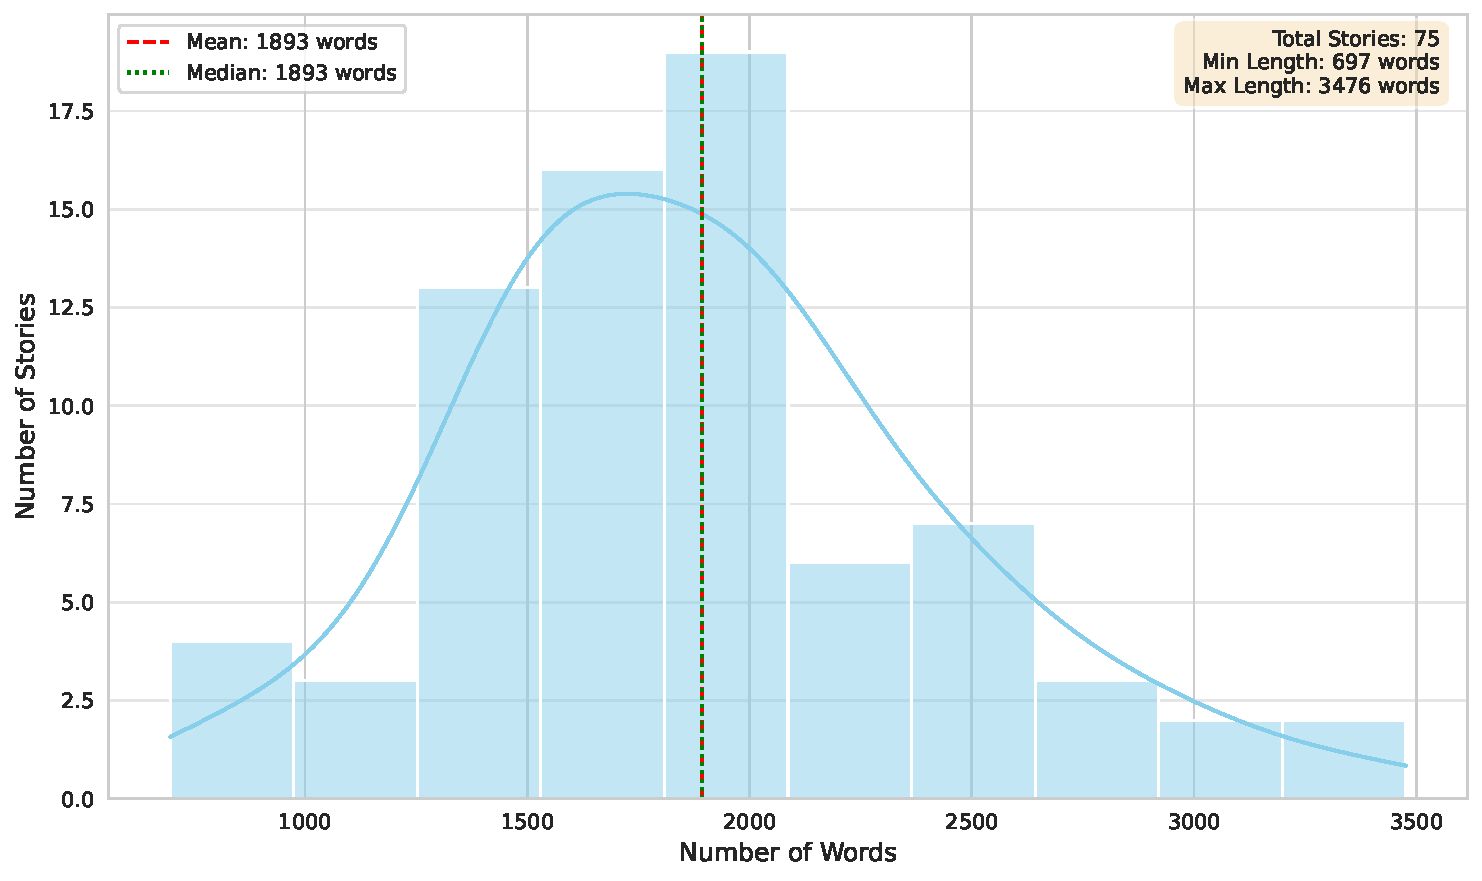
\includegraphics[width=0.8\textwidth]{figs/story_length_distribution.pdf}
    \caption{Distribution of story lengths in training/validation dataset.}
    \label{fig:story_length}
\end{figure}

The following shows a selected piece of one of the stories. The punctuations are added by us as it is not in the original text.

\begin{quotation}
    "My story begins, I am driving my uh silver station Volvo uh from Brooklyn to my mother's house in Rosedale, Queens, on a hot mid-afternoon August day in two thousand and three. My mother uh is a widow. Uh, my father has passed away from lung cancer fifteen years before, nineteen eighty-eight, and she has not resumed dating. She has sworn off men in no uncertain terms. She has told me that, "I am never, ever going to wash another pair of men's underwear again. I am finished with the species. I'm done."
\end{quotation}

The story is a narrative piece, and the text is rich in detail and context. The language is conversational, with a mix of personal anecdotes and reflections. The use of "uh" indicates a speech pattern that is common in spoken language. That implies the corpus is informal and could differ from more formal ones that commonly used in NLP-related tasks.

\subsection{fMRI Signals}
The fMRI signal data captures the brain's response, measured via the Blood-Oxygen-Level-Dependent (BOLD) signal, as subjects listened to the stories. For each of the 75 stories comprising the training/validation set for a given subject, the data is organized into a two-dimensional numerical array. Each row in this array represents the brain activity across all measured voxels at a specific Time of Repetition (TR), which is the sampling interval of the fMRI scanner. Each column corresponds to a single voxel, with 94251 voxels for Subject 2 or 95556 for Subject 3, recorded per subject. Consequently, the dimensions of these arrays are \(T \times V\), where \(V\) is constant, and \(T\) (the number of TRs) varies from story to story, reflecting the differing lengths of the narratives; indeed, as shown in Figure \ref{fig:word_count}, there is a strong positive correlation between the number of words in a story and the duration of its corresponding fMRI recording in TRs.

\begin{figure}[ht]
    \centering
    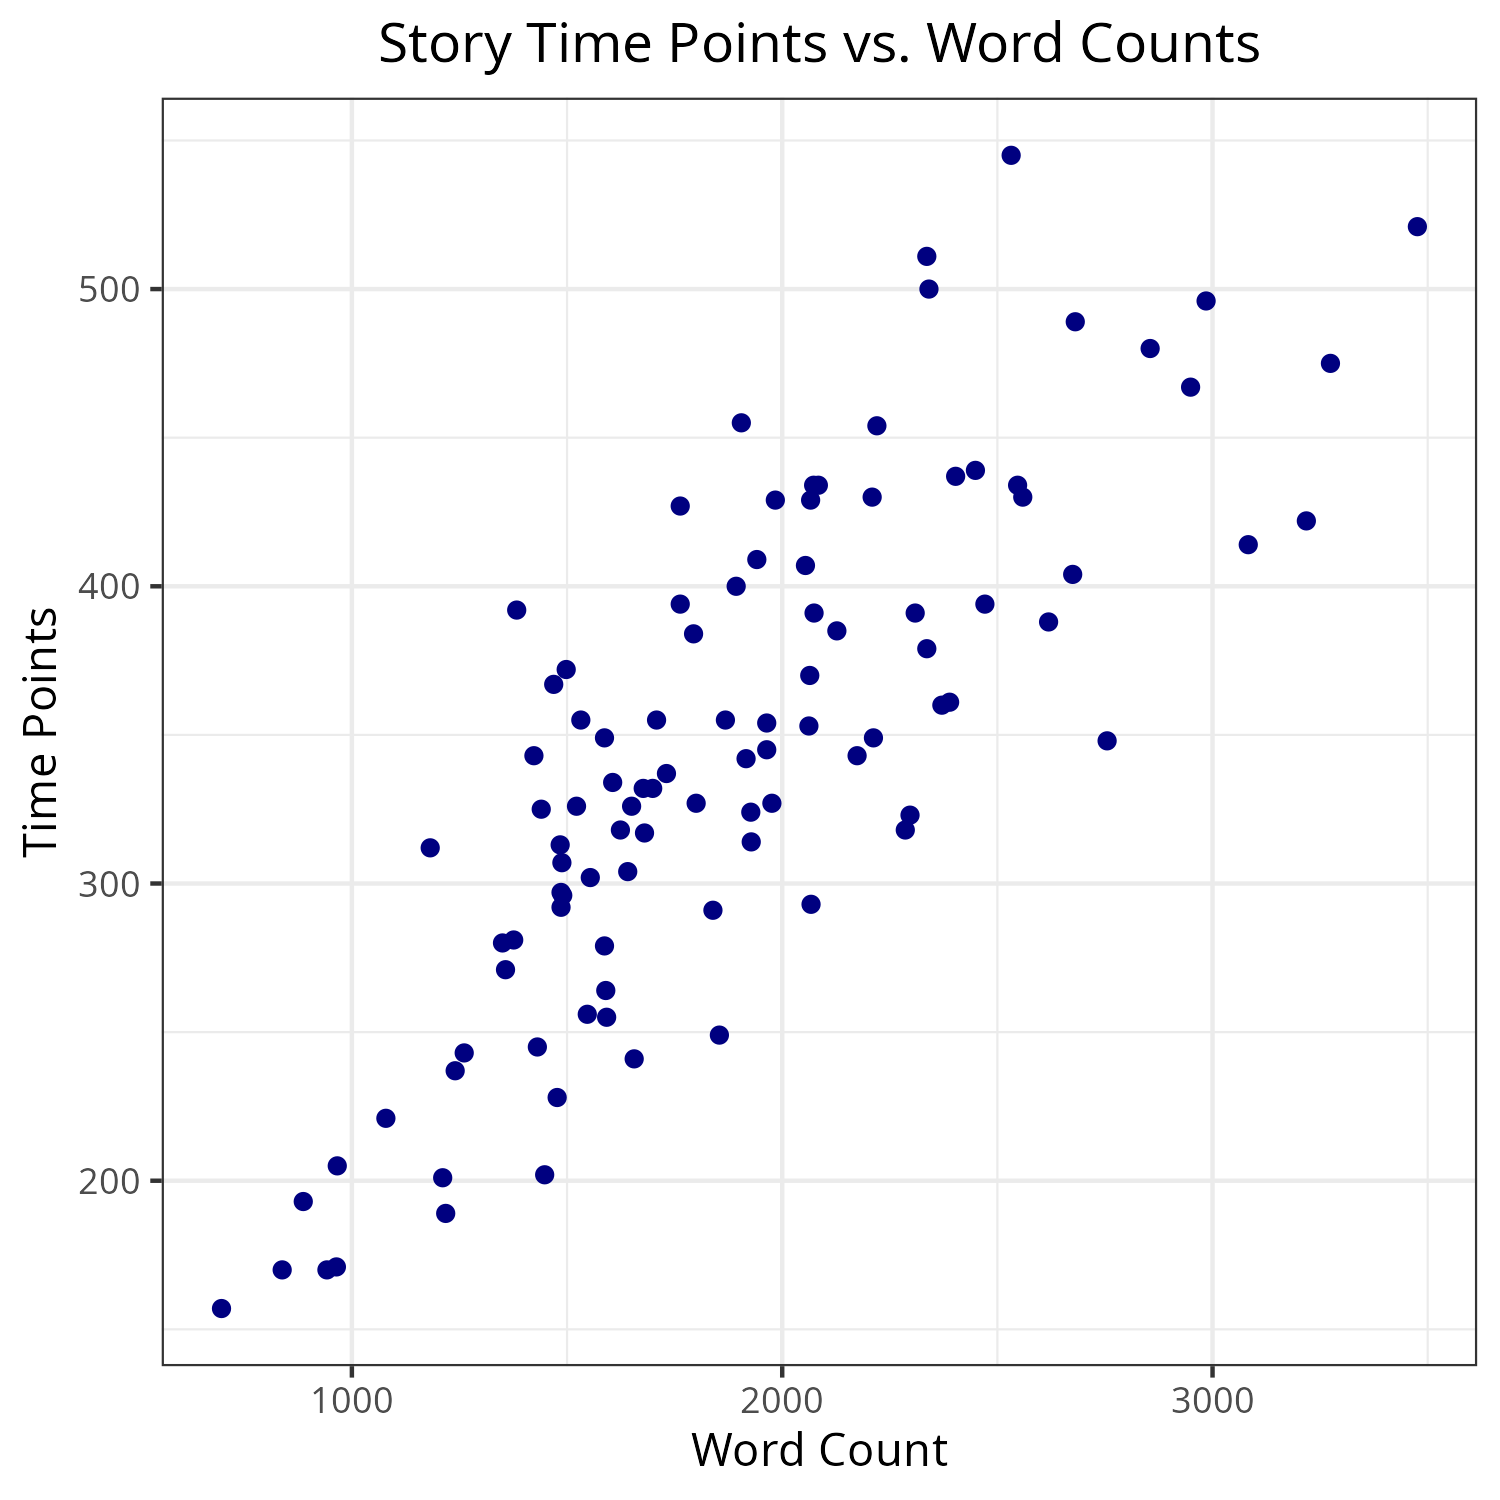
\includegraphics[width=0.6\textwidth]{figs/word_count.png}
    \caption{The number of words in a story is strongly correlated with the number of fMRI repetition time points.}
    \label{fig:word_count}
\end{figure}

To understand the basic characteristics of the BOLD signal itself, we examined the distribution of raw signal values across all voxels and time points within the training/validation set. Since plotting every single reading is impractical, we randomly sampled 10,000 individual signal values from the training data for each subject. Figure \ref{fig:fmri_signal} displays the resulting histograms for these sampled raw BOLD values for Subject 2 and Subject 3. Both distributions appear highly similar, exhibiting an unimodal, approximately Gaussian form centered very close to zero. The spread or variance of the raw signals also seems comparable between the two subjects.

\begin{figure}[ht]
    \centering
    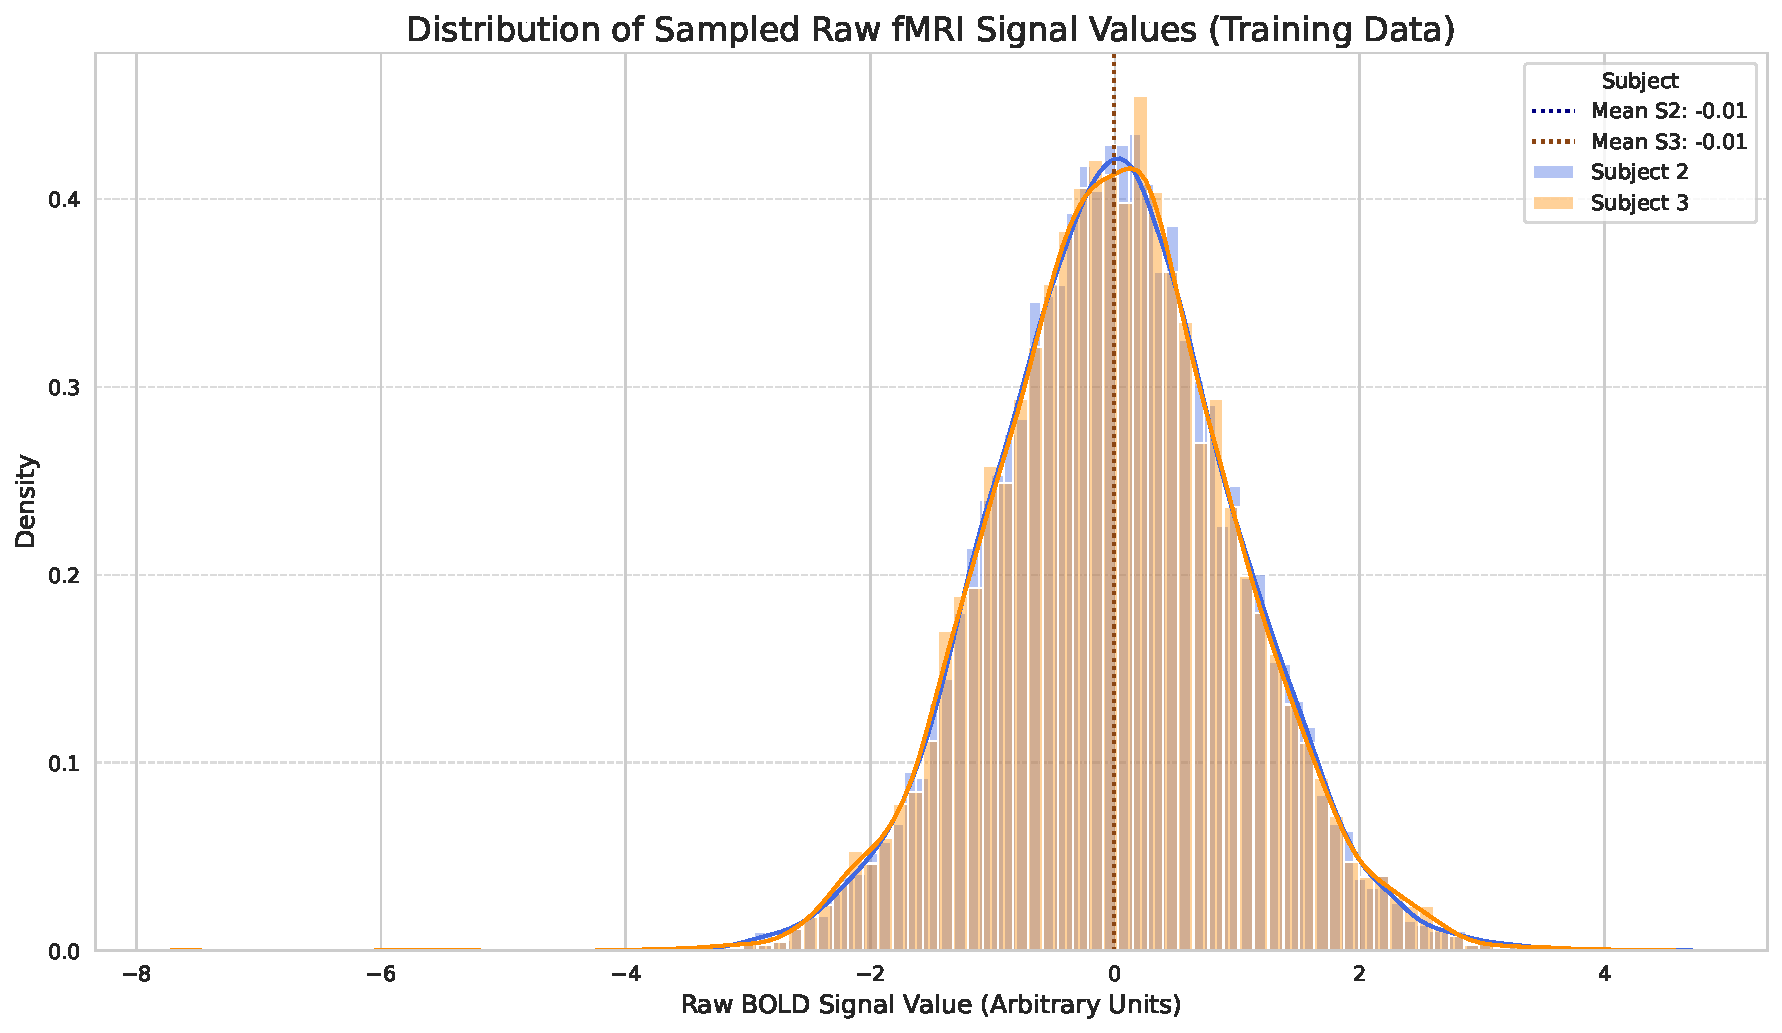
\includegraphics[width=0.8\textwidth]{figs/fmri_signal_distribution.pdf}
    \caption{Distribution of fMRI signals in training/validation dataset.}
    \label{fig:fmri_signal}
\end{figure}

In addition to examining the average fMRI signal across the entire dataset, it is informative to visualize the distribution of signals for each story individually. Figure \ref{fig:boxplots} presents the distribution of several summary statistics (mean, median, interquartile range (IQR), minimum, and maximum) computed from the fMRI signal for each of the 101 stories, where each story is treated as a single data point. The central tendency and spread (IQR) appear highly consistent across stories, while the minimum and maximum values show much greater variability. This variation in extremes may reflect story-specific events or transient noise artifacts.

\begin{figure}[ht]
    \centering
    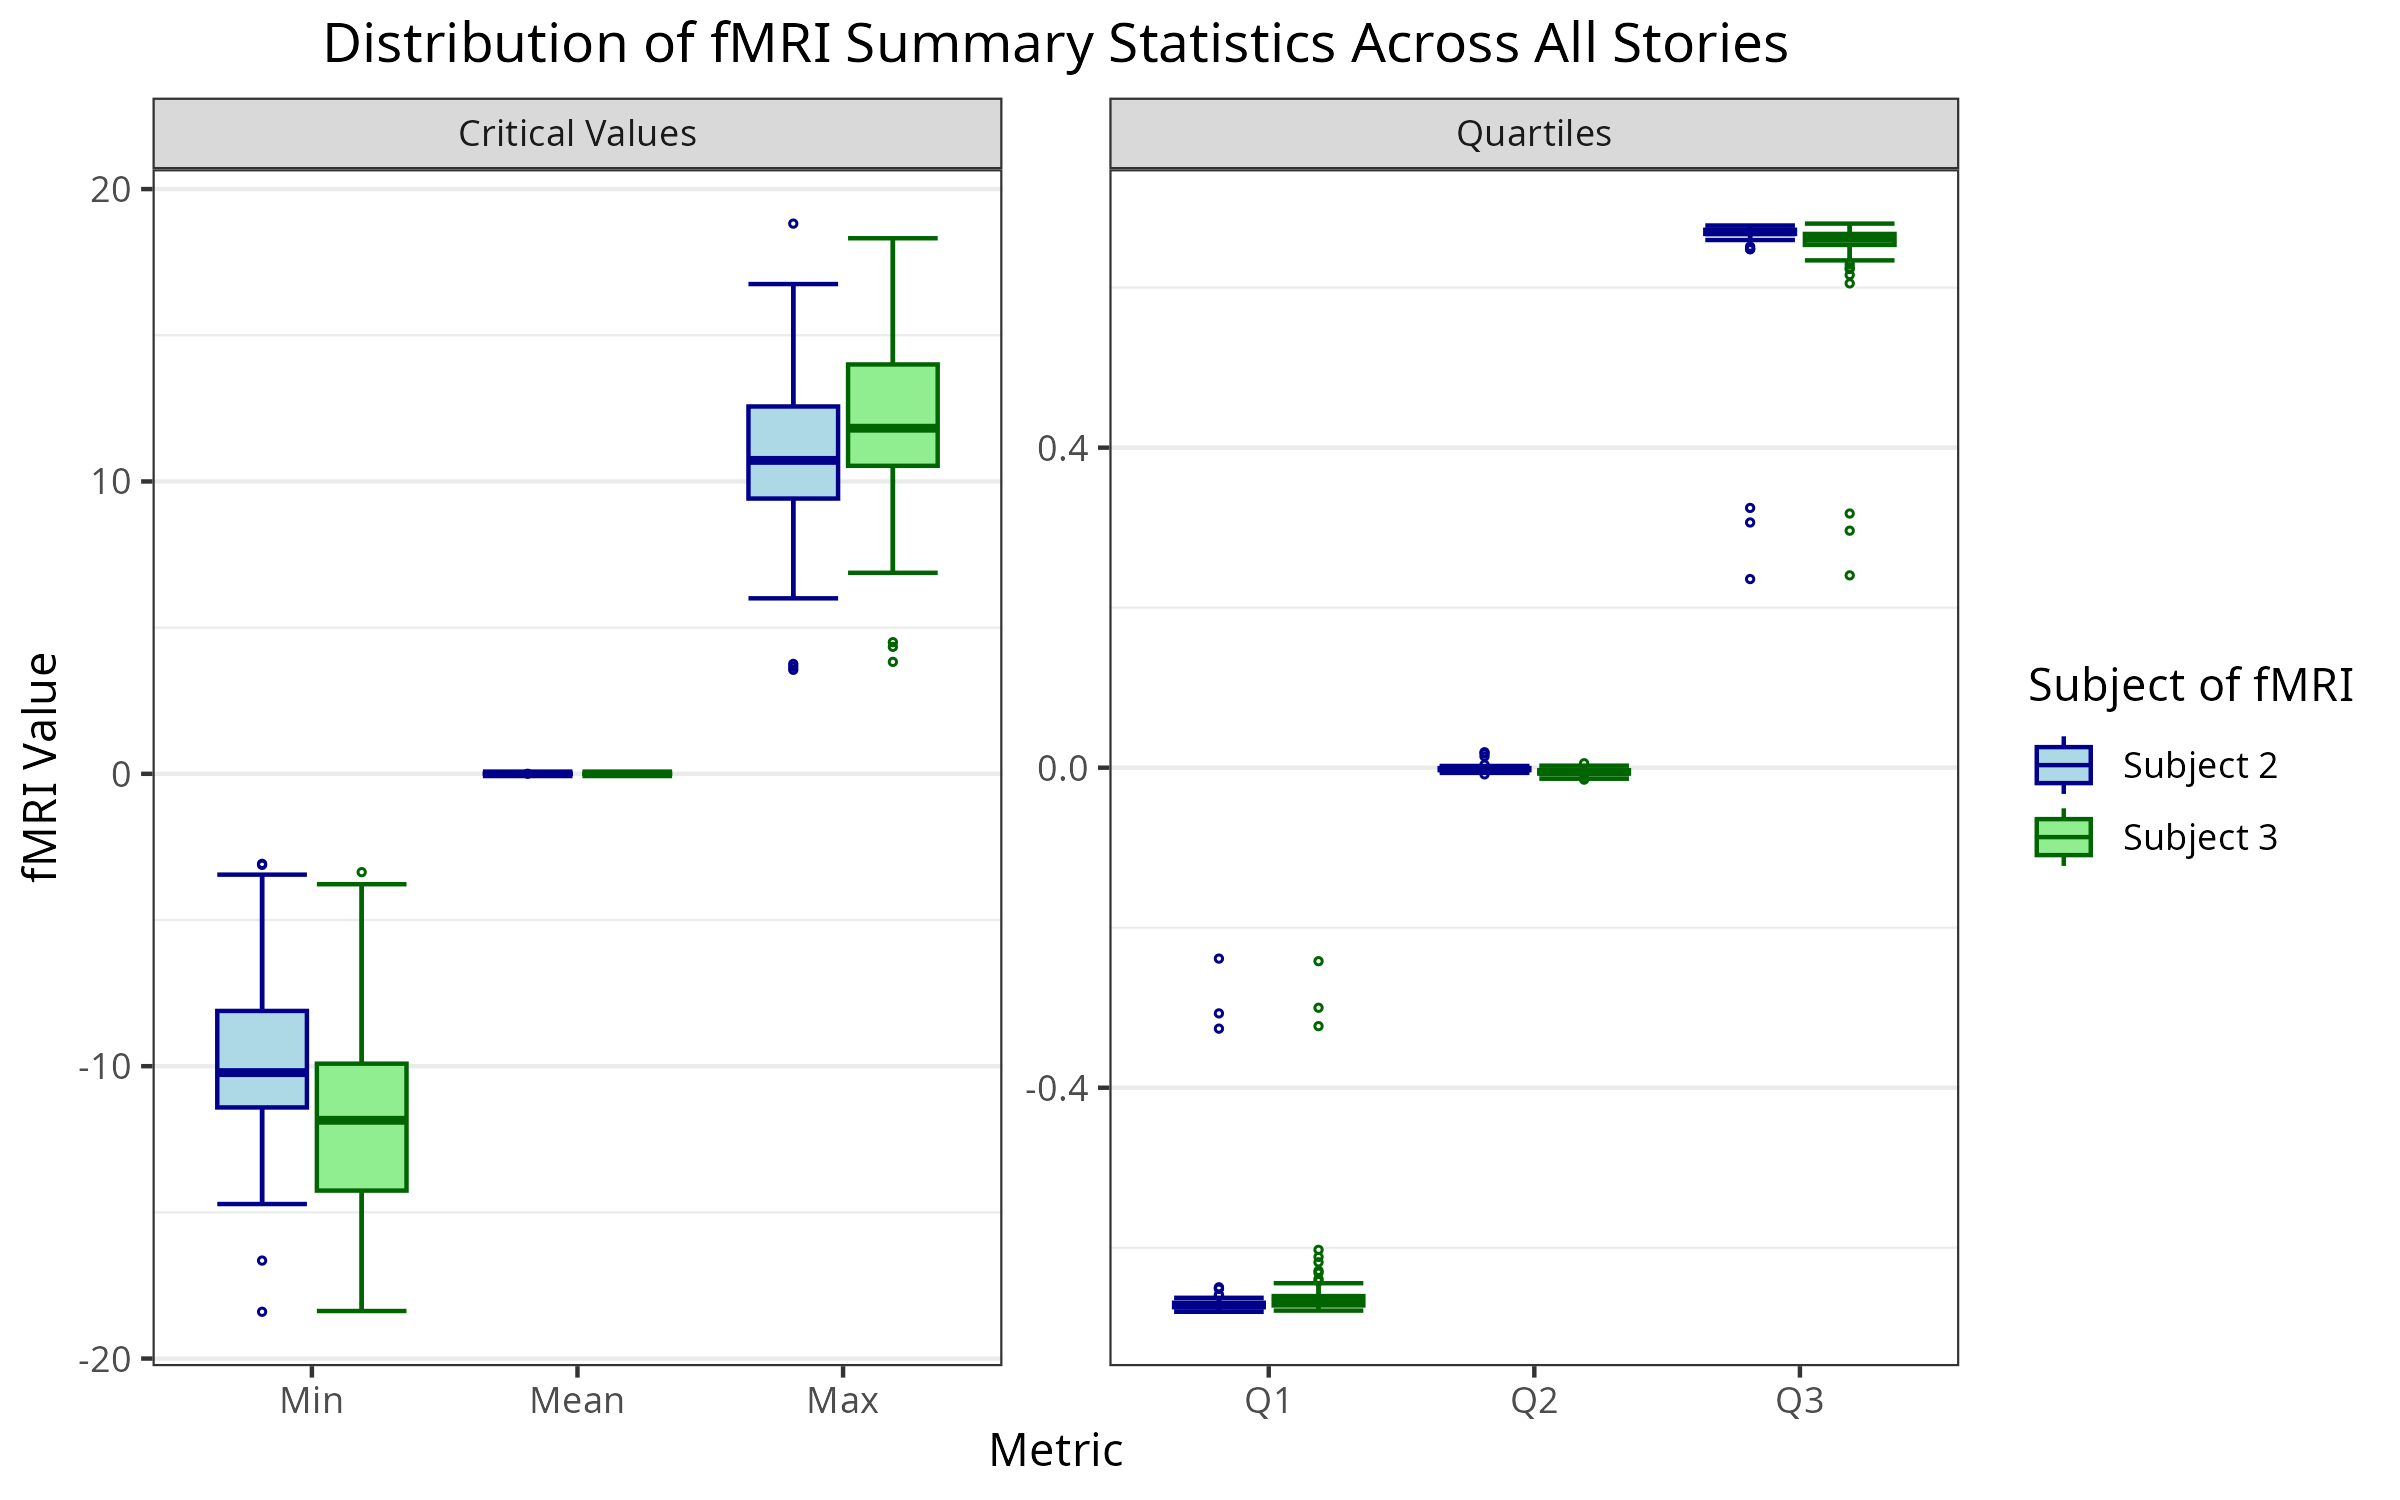
\includegraphics[width=0.8\textwidth]{figs/boxplots.png}
    \caption{Across all 101 stories, the mean, median, and interquartile range (Q1–Q3) of fMRI signals are tightly distributed, while the minima and maxima show wide variation.}
    \label{fig:boxplots}
\end{figure}

Figure \ref{fig:mean_signal} offers a more granular view by plotting the mean and IQR of the fMRI signal across all voxels at each time point within selected example stories. This enables a direct comparison of the temporal signal profiles between Subject 2 and Subject 3 over the course of each story. Despite some fluctuations, the mean signal values for both subjects consistently oscillate within a relatively narrow range (approximately –1 to 1), not only in the stories shown here but across the full set.

\begin{figure}[ht]
    \centering
    \parbox{\textwidth}{\centering 
        \fontsize{13pt}{13pt}\selectfont \textbf{Average fMRI Signal Across Selected Stories}  
        {\fontsize{11pt}{13pt}\selectfont Mean (line) and IQR (shaded) comparison between   \textcolor{RoyalBlue}{\textbf{Subject 2}} and \textcolor{ForestGreen}{\textbf{Subject 3}}.} 
    }
    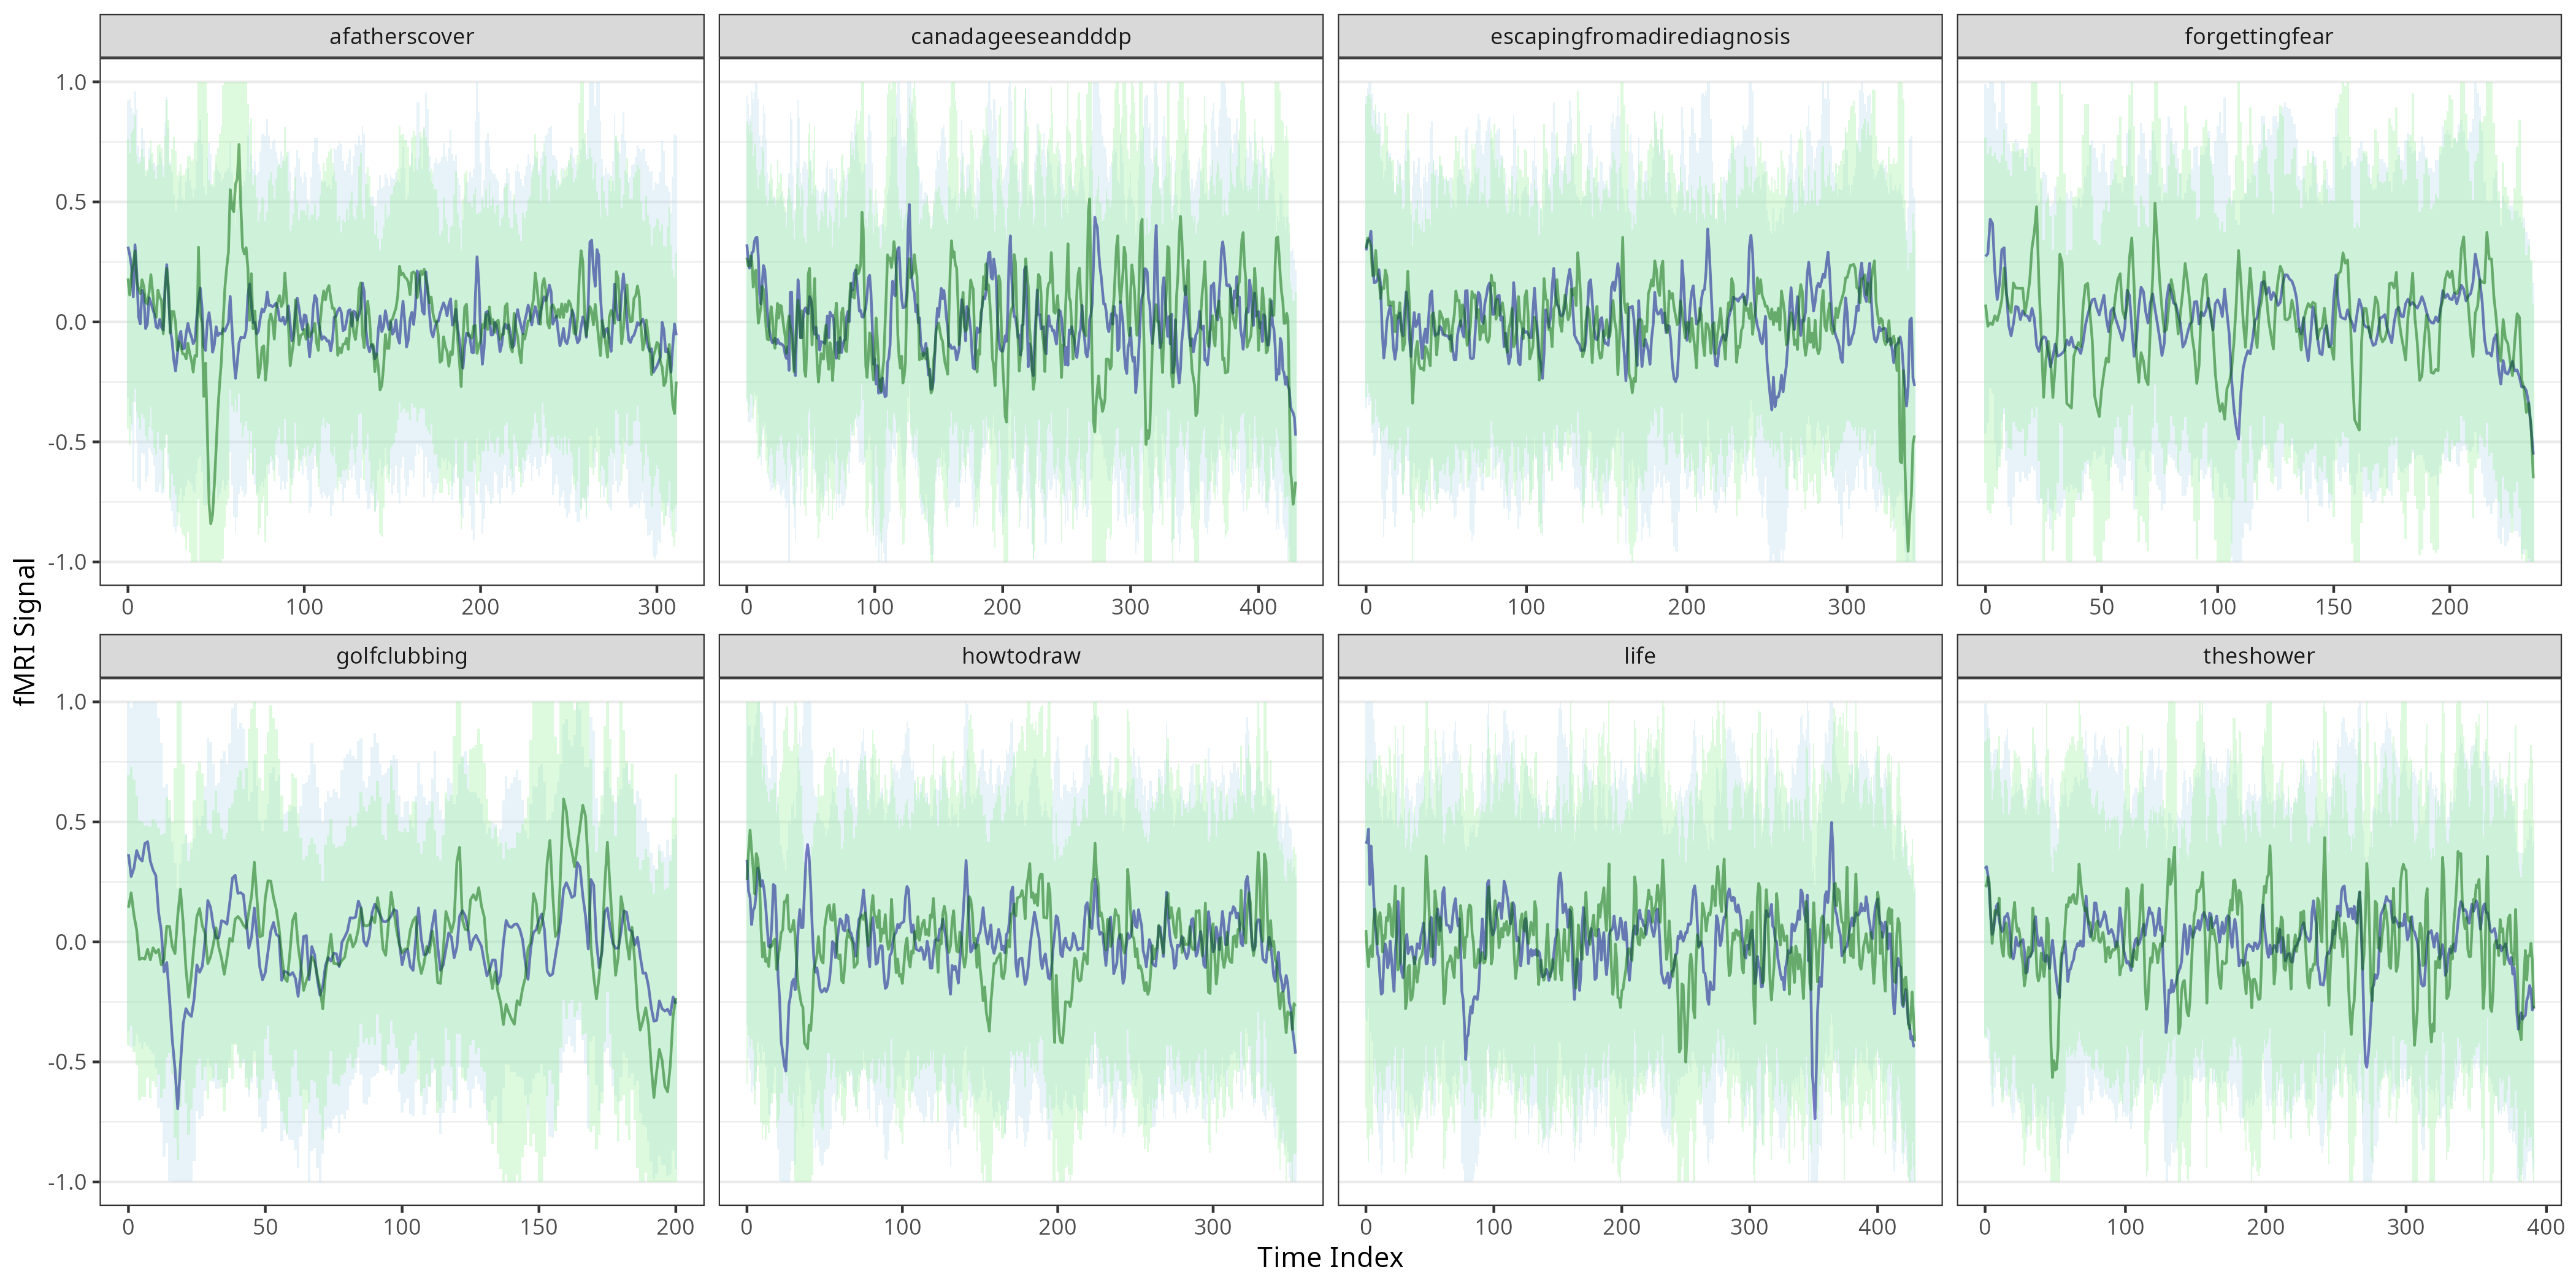
\includegraphics[width=\textwidth]{figs/mean_signal.png}
    \caption{Mean fMRI signal (line) and interquartile range (shaded area) for Subject 2 and Subject 3 at each time point, plotted separately for each story. Mean values for both subjects generally oscillate between –1 and 1.}
    \label{fig:mean_signal}
\end{figure}

In stark contrast, the maximum signal value at each time point, shown in Figure~\ref{fig:max_signal}, reveals substantial variability in peak activity levels over the course of a single story. Although some of this variation may be driven by noise, there appears to be a moderate degree of correlation or shared structure in the timing of peak signal fluctuations between the two subjects listening to the same story.

\begin{figure}[ht]
    \centering
    \parbox{\textwidth}{\centering 
        \fontsize{13pt}{13pt}\selectfont \textbf{Maximum fMRI Signal Across Selected Stories}  

        {\fontsize{11pt}{13pt}\selectfont Comparison between \textcolor{RoyalBlue}{\textbf{Subject 2}} and \textcolor{ForestGreen}{\textbf{Subject 3}}.} 
    }
    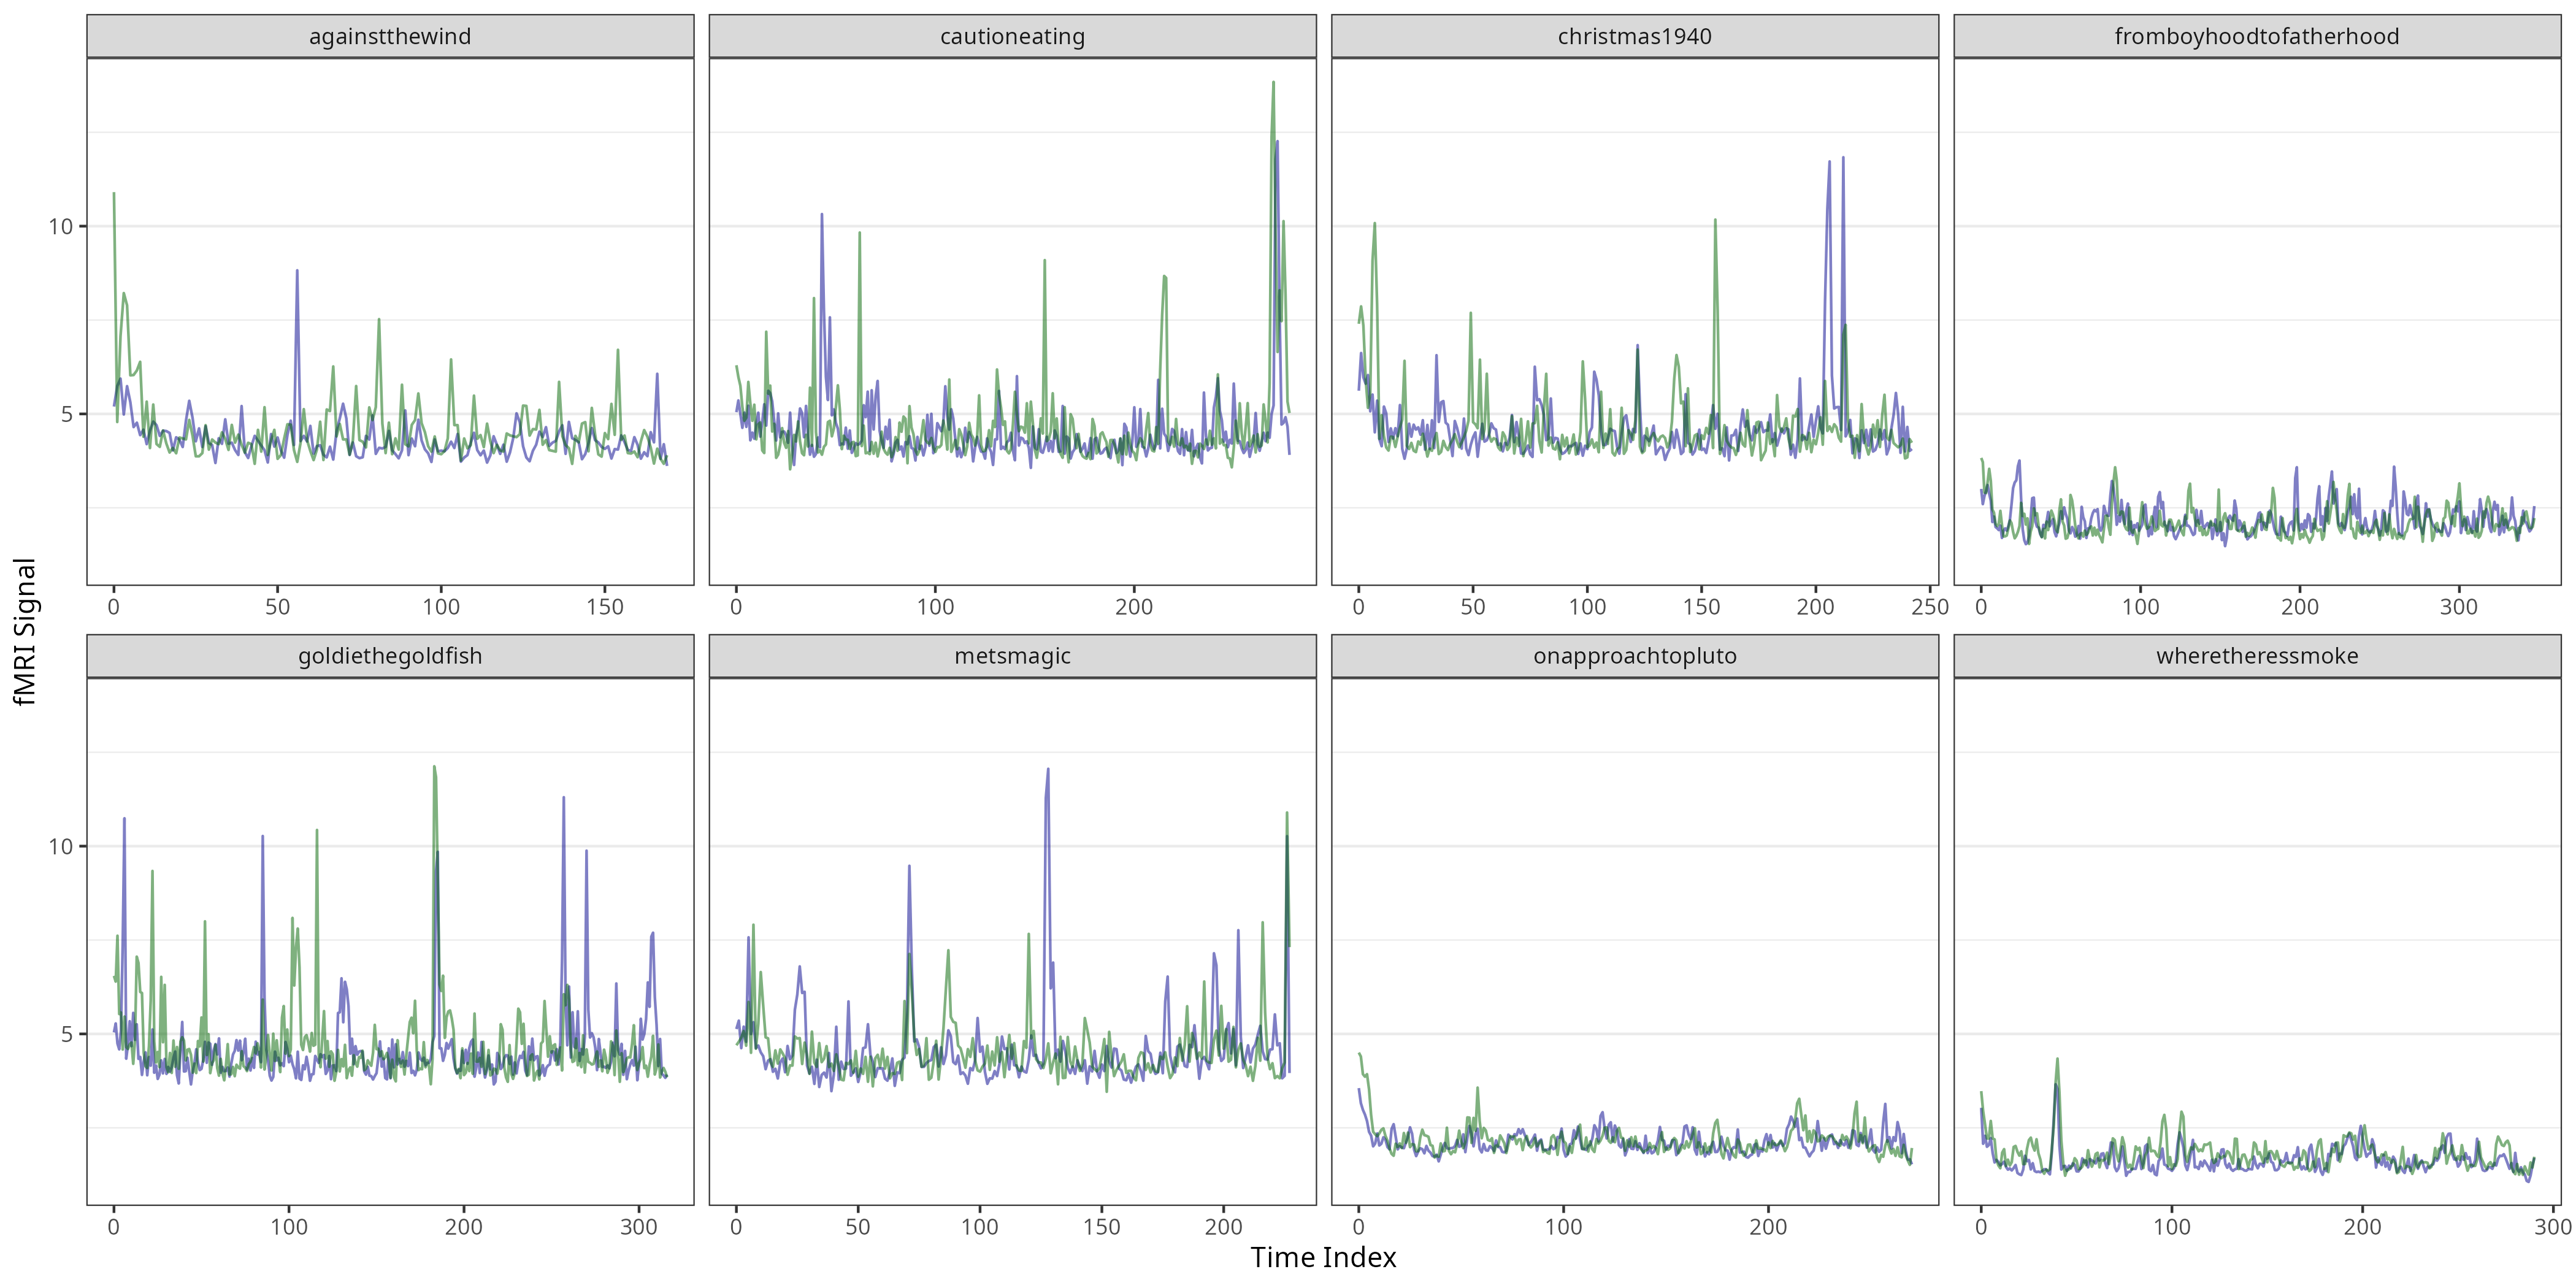
\includegraphics[width=\textwidth]{figs/max_signal.png}
    \caption{Maximum fMRI signals for Subject 2 and Subject 3 are highly moderate across several stories, despite substantial noise.}
    \label{fig:max_signal}
\end{figure}

Another thing to note is that the fMRI signals of Subject 2 contain some NaN values, which are not present in Subject 3. However, the proportion of NaN values is very small, only \(5.9 \times 10^{-6}\) of the total number of values. Due to the small proportion, we simply imputed them with the global mean to prepare the prediction and expect no significant impact on the model performance no matter which imputation method we use.

\section{Embeddings}
To predict brain activity (fMRI signals) from the podcast stimuli the subjects listened to, we first need to convert the raw text of the stories into a numerical format suitable for machine learning models. This conversion is achieved through text embeddings, representing text as dense vectors. In Lab 3.1, we explored word-level methods like Bag-of-Words and pre-trained Word2Vec/GloVe embeddings. For Lab 3.2, our primary focus shifts to generating custom embeddings with a self-trained BERT \cite{devlin2019bert}. We implement and pre-train an encoder-only Transformer-based \cite{vaswani2017attention} BERT model using the Masked Language Modeling (MLM) objective. This involves training the model to predict randomly masked tokens within the story text, forcing it to learn rich contextual representations. We utilize the pre-trained tokenizer in the original BERT to prepare the text data. The resulting encoder, trained on the stories, is then used to generate embeddings for each word in the stories. These custom embeddings, after undergoing downsampling and temporal delay processing similar to Lab 3.1, will serve as the input features for the subsequent ridge regression analysis aimed at predicting voxel activity.

\subsection{BERT Pre-training}
We pre-train a BERT-like model on the training/validation stories using the MLM objective, as specified in the lab instructions. In this subsection, we provide a detailed overview of the pre-training process, including the tokenization of the text data, the architecture of the BERT model, the training procedure, and the motivation behind the chosen design choices.

\subsubsection{Tokenization and Token Embedding}
The first step in the pre-training process is to tokenize the text data. We utilize the pre-trained BERT tokenizer in the original BERT implementation \cite{devlin2019bert} as instructed (the bert-base-uncased in Huggingface's transformers library \cite{wolf2019huggingface}). This tokenizer is a subword tokenizer that splits words into smaller subword units, but never represents multiple words as a single token, nor does it include both characters and spaces/punctuation in the same token, unlike a modern LLM tokenizer. However, it still handles out-of-vocabulary words by breaking them down into subword units, allowing the model to learn representations for rare or unseen words. The tokenizer also adds special tokens, specifically [CLS] at the beginning of the sequence and [SEP] at the end. The tokenization process converts the raw text into a sequence of token IDs, which are then used as input to the BERT model.

After converting the text into token IDs, we embed them into dense vectors using the pre-trained BERT embedding layer in the original BERT model. The reason for using the pre-trained embedding layer is that the training data is too small, and we will have many out-of-vocabulary words in the new stories if we train the embedding layer from scratch. The pre-trained embedding layer has a dimensionality of 768, which is too large for our dataset and is likely to introduce overfitting. Therefore, we reduce the dimensionality of the embeddings to our embedding dimension (a hyperparameter will be chosen later) using a linear layer with trainable weights while the BERT embedding layer is frozen. This allows us to learn a lower-dimensional representation of the input tokens while still leveraging the pre-trained knowledge from the original BERT model.

\subsubsection{BERT Architecture}
The original BERT model was proposed in 2018, and many improvements in the backbone transformer architecture have been made since then. In this lab, we use a modernized transformer architecture based on LLaMA 3 \cite{grattafiori2024llama}, with some modifications. The details of the architecture are as follows.

\begin{itemize}
    \item \textbf{Embedding Dimension:} 32 or 64.
    \item \textbf{Hidden Dimension:} 112 for embedding dimension 32, and 224 for embedding dimension 64.
    \item \textbf{Number of Layers:} 2.
    \item \textbf{Attention Type:} Bidirectional Multi-Head Attention.
    \item \textbf{Number of Attention Heads:} 4.
    \item \textbf{Activation Function:} SwiGLU \cite{shazeer2020glu}.
    \item \textbf{Bias:} No bias in the attention and feed-forward layers.
    \item \textbf{Normalization:} pre-layer Root Mean Square Layer Normalization \cite{zhang2019root} with epsilon set to \(1 \times 10^{-5}\) applied before the attention and feed-forward layers.
    \item \textbf{Positional Embedding:} Rotary Position Embedding (RoPE) \cite{su2024roformer} with theta parameter set to 500000.
\end{itemize}

The selection of these hyperparameters aims to build a lightweight model that can be trained on the limited amount of data available in the stories while incorporating modern techniques to improve performance. The embedding dimension, hidden dimension, number of attention heads, and number of layers are kept small to reduce the model size. The SwiGLU activation function, Root Mean Square Layer Normalization, No Bias, and Rotary Position Embedding (RoPE) are modern techniques that have been shown to improve performance in transformer models. Besides, the RoPE enables the model to be trained on longer sequences without adding additional parameters and be applied to longer sequences than the training data. The epsilon parameter in the normalization layer is set to \(1 \times 10^{-5}\) to align with LLaMA 3's implementation. Finally, bidirectional multi-head attention is necessary to train a BERT-like model, as it allows the model to attend to past and future tokens in the input sequence.

Okay, here is a draft for the `Training Procedure` subsection, following the structure of the `BERT Architecture` section.

\subsubsection{Training Procedure}
The encoder model was pre-trained using the Masked Language Modeling (MLM) objective, a standard self-supervised learning technique for training BERT-like models \cite{devlin2019bert}. The specific details of the training setup are outlined below:

\begin{itemize}
    \item \textbf{Objective:} Masked Language Modeling (MLM) only.
    \item \textbf{Loss Function:} Cross-Entropy loss, calculated only between the model's predictions and the true token IDs for the positions that were masked in the input sequence.
    \item \textbf{Masking Strategy:} Input tokens were randomly selected for masking with a probability of 0.1, 0.15, or 0.2 (varied as a hyperparameter). Following the original BERT strategy:
    \begin{itemize}
        \item 80\% of selected tokens were replaced with a special [MASK] token.
        \item 10\% were replaced with a random token from the vocabulary.
        \item 10\% were left unchanged.
    \end{itemize}
    Padding tokens were never masked.
    \item \textbf{Sequence Length:} No limit on the maximum sequence length thus we use a whole story as a single sequence. The longest sequence in the training data is 3586 tokens, and the model can handle sequences longer than this.
    \item \textbf{Optimizer:} AdamW \cite{loshchilov2017decoupled}.
    \item \textbf{Base Learning Rate:} \(1 \times 10^{-3}\) scaled relative to a reference batch size of 75 with a linear scaling rule.
    \item \textbf{Learning Rate Schedule:} Linear warmup for the first 50 epochs, followed by a cosine decay down to a minimum learning rate of \(1 \times 10^{-4}\).
    \item \textbf{Training Epochs:} Total Training Epochs: 1000. Checkpoints saved at epochs: 0, 100, 200, ..., 1000.
    \item \textbf{Batch Size:} 25.
    \item \textbf{Gradient Clipping:} Gradients were clipped to a maximum L2 norm of 1.0.
    \item \textbf{Mixed Precision:} Automatic Mixed Precision was enabled with bfloat16 to accelerate training and reduce memory usage.
\end{itemize}

The training procedure was designed to pre-train the custom encoder on the podcast text corpus. We use the MLM objective only, while the original BERT model also uses the Next Sentence Prediction (NSP) objective. However, later research has shown that the NSP objective does not significantly improve performance on downstream tasks \cite{liu2019roberta}. We experiment with masking probabilities of 0.1, 0.15, and 0.2 to find the optimal balance for this dataset (a hyperparameter). The 80/10/10 replacement strategy is adopted directly from the original BERT methodology.

Unlike the original BERT which has a maximum sequence length of 512 tokens, we do not impose a maximum sequence length on the input sequences. This stems from RoPE's parameterless nature, which allows the model to handle longer sequences without growing the model size. Besides, the longest sequence in the training data is 3586 tokens, which is not excessively long and computationally feasible given the small size of the model and the limited amount of training data. The model can also be applied to longer sequences than the training data, which is a desirable property.

The optimizer, learning rate (and schedule), gradient clipping, and Automatic Mixed Precision Training follow standard practices for training transformer models. The batch size is chosen to be as large as possible given the limited GPU memory available.

Finally, we train the model for 1000 epochs and save a checkpoint every 100 epochs. 6 models are trained in total, with different embedding dimensions (32 and 64) and different masking probabilities (0.1, 0.15, and 0.2). The loss curves for the training data are shown in Figure \ref{fig:loss_curves}. As expected, larger embedding dimensions and lower masking probabilities lead to lower training loss.

\begin{figure}[ht]
    \centering
    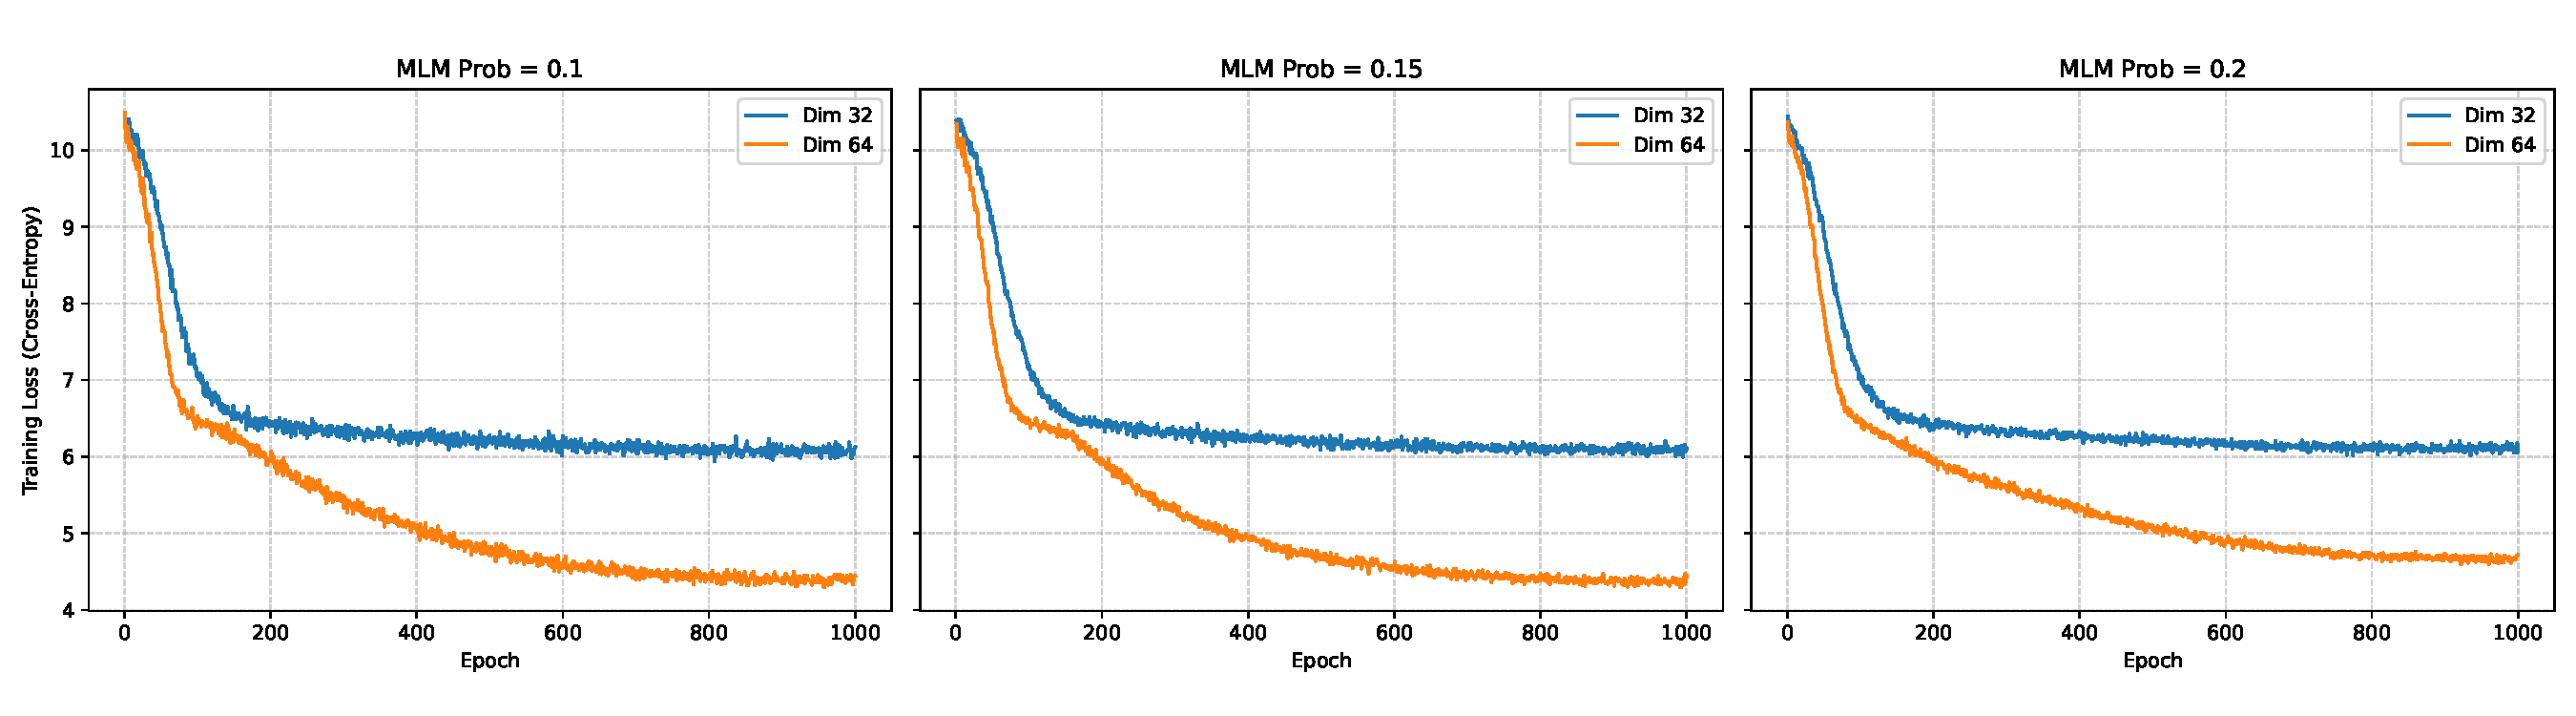
\includegraphics[width=\textwidth]{figs/training_loss_comparison.pdf}
    \caption{Comparison of Training Loss Across Model Dimensions and MLM Probabilities. The loss value is per masked token.}
    \label{fig:loss_curves}
\end{figure}

We do not use a validation set for the pre-training process. Instead, we train the model on the whole training/validation set. This is because the training/validation set is small, and we want to leverage all available data for pre-training. Moreover, the validation loss for the MLM objective is not a good indicator of the model's performance on downstream tasks, so we will make the final decision on the best model based on the downstream task performance in the following Modeling section instead. To mimic the potential validation loss-based early stopping process, we save the model every 100 epochs and evaluate all the saved models on the downstream task to mitigate the risk of overfitting due to long training.

\subsection{Extracting Word Embeddings}
After pre-training the BERT model, we extract the word embeddings for each word in the stories. The subword tokenizer never represents multiple words as a single token, nor does it include both characters and spaces/punctuation in the same token. Therefore, for words represented by a single token, we can directly use the corresponding final hidden state output of the encoder model as the word embedding. For words represented by multiple tokens, we take the average of the embeddings of the subword tokens to obtain a single-word embedding. In the embedding extraction process, we also remove the special tokens [CLS] and [SEP] added by the tokenizer.

We feed the entire token sequence for a story into the trained encoder model simultaneously. This process generates output embeddings (final hidden states) where the representation for each token is influenced by all other tokens in the story. Consequently, although we ultimately derive an embedding for each individual word (using the single-token or averaging approach described above), each word's vector inherently captures the rich contextual information provided by the full narrative. This stands in contrast to the context-agnostic methods used in Lab 3.1.


\subsection{Chunk-level Aggregation with Lanczos Resampling}

The word-level embeddings generated in the previous step provide a representation for each word occurring at specific time points in the story. However, the fMRI signals we aim to predict are measured at discrete time intervals, known as Repetition Times (TRs). During a single TR, multiple words may be presented to the subject. Therefore, the sequence of word embeddings (with dimensions \(\text{num\_words} \times \text{embedding\_dim}\)) needs to be aggregated to match the temporal resolution of the fMRI data, resulting in a single embedding vector for each TR (dimensions \(\text{num\_TRs} \times \text{embedding\_dim}\)).

To achieve this temporal alignment and aggregation, we employ Lanczos interpolation, given in the instruction, a commonly used technique for signal resampling. This method calculates the embedding representation for each TR time point by applying a weighted average (convolution) to the surrounding word-level embeddings. The weights are determined by the Lanczos kernel, which is a windowed sinc function. Specifically, the weight assigned to a word embedding at time \(t_{word}\) when calculating the aggregated embedding for TR center time 
\(t_{TR}\) is given by the Lanczos kernel function \(L(t)\):

\[
L(t) = \text{sinc}(\pi t f_c) \cdot \text{sinc}(\frac{\pi t f_c}{a}) \cdot \mathbb{I}(|t f_c| < a)
\]

where \(t = t_{TR} - t_{word}\) is the time difference, $f_c$ is the cutoff frequency, $a$ is the window size parameter, and \(\text{sinc}(x) = \frac{\sin(x)}{x}\).

In signal processing, the Lanczos kernel minimizes aliasing artifacts that can arise when downsampling and provides a good balance between smoothing noise and preserving the relevant temporal structure, compared to simpler methods like rectangular window averaging or nearest-neighbor interpolation. Applying the Lanczos kernel on word sequences is heuristic because the word embeddings are not continuous, and dramatically changing in a short time is reasonable and expected. However, it still provides an effective way to aggregate the word-level embeddings into chunk-level representations that align with the fMRI TRs.

\subsection{Temporal Feature Engineering}
In Lab 3.1, because the embedding methods are context-agnostic, temporal feature engineering is necessary to capture the temporal dependencies in the data. However, in this lab, BERT embeddings are context-aware, so we do not need to perform temporal feature engineering on the embeddings explicitly. Thus, we use the raw BERT embeddings directly as the input features for the modeling step. But in Section 4, where the same method as Lab 3.1 is applied, we use the same temporal feature engineering methods as in Lab 3.1.

\section{Modeling - Pre-Trained Embeddings}

\subsection{Modeling Approach}
We create a predictive model to predict fMRI levels for each voxel using the pre-trained embeddings we have generated. Specifically, we fit a ridge regression model. This modeling approach contains the parameter alpha, which controls the penalty term on the model's weights as L2 (squared) loss.

We start by fitting a regression model for Subject 2, for each different embedding - Bag of Words, GloVe, and Word2Vec. Using the cross-validation strategy described in the next section, we find the best alpha hyperparameter value for regularization.

\subsection{Model Evaluation Strategy}

We utilize a standard k-fold cross-validation strategy to develop our predictive models. The split is done at a story level instead of a TR level to mimic the real-world scenario where the model is trained on a set of stories and then evaluated on unseen stories. 60\% of the stories are used for training and validation, and the remaining are reserved for testing and remain untouched until the final evaluation.

For each fold, the bag-of-words is retrained on the training data to avoid data leakage, while the pre-trained embeddings are applied before the data split as they are fixed and independent of the training data.

The metric we use to evaluate the model performance is the correlation coefficient (CC) between the predicted and actual fMRI signals, which is a standard metric in the context of fMRI signals. We do this per voxel, giving us a voxel-wise CC. This is the metric that our model is trained to optimize for.

This strategy is designed to mimic the real-world scenario with the best efforts to avoid data leakage and measure the model's generalization performance.

\subsection{Results}

Our cross-validation results for hyperparameter tuning are shown in Tables \ref{tab:word2vec_cv}, \ref{tab:glove_cv}, and \ref{tab:bow_cv} for the models trained with the Word2Vec, GloVe, and Bag of Words embeddings, respectively. These are performance metrics on the validation set.


\begin{table}[ht]
\centering
\caption{Performance metrics for Word2Vec at different values of \texttt{alpha}. Best alpha: 1000 (Mean CV CC = 0.0057).}
\label{tab:word2vec_cv}
\begin{tabular}{rrrrr}
\toprule
\textbf{Alpha} & \textbf{Mean CC} & \textbf{Median CC} & \textbf{Top1 CC} & \textbf{Top5 CC} \\
\midrule
0.1    & 0.0035 & 0.0032 & 0.0462 & 0.0325 \\
1      & 0.0036 & 0.0032 & 0.0462 & 0.0325 \\
10     & 0.0036 & 0.0032 & 0.0463 & 0.0325 \\
100    & 0.0039 & 0.0035 & 0.0478 & 0.0330 \\
1000   & 0.0057 & 0.0051 & 0.0518 & 0.0364 \\
\bottomrule
\end{tabular}
\end{table}

\begin{table}[ht]
\centering
\caption{Performance metrics for GloVe at different values of \texttt{alpha}. Best alpha: 1000 (Mean CV CC = 0.0067).}
\label{tab:glove_cv}
\begin{tabular}{rrrrr}
\toprule
\textbf{Alpha} & \textbf{Mean CC} & \textbf{Median CC} & \textbf{Top1 CC} & \textbf{Top5 CC} \\
\midrule
0.1    & 0.0048 & 0.0044 & 0.0474 & 0.0337 \\
1      & 0.0048 & 0.0044 & 0.0474 & 0.0337 \\
10     & 0.0058 & 0.0046 & 0.0479 & 0.0341 \\
100    & 0.0055 & 0.0051 & 0.0496 & 0.0352 \\
1000   & 0.0067 & 0.0061 & 0.0535 & 0.0377 \\
\bottomrule
\end{tabular}
\end{table}

\begin{table}[ht]
\centering
\caption{Performance metrics for BoW at different values of \texttt{alpha}. Best alpha: 1000 (Mean CV CC = 0.0230).}
\label{tab:bow_cv}
\begin{tabular}{rrrrr}
\toprule
\textbf{Alpha} & \textbf{Mean CC} & \textbf{Median CC} & \textbf{Top1 CC} & \textbf{Top5 CC} \\
\midrule
0.1    & 0.0063 & 0.0062 & 0.0451 & 0.0338 \\
1      & 0.0084 & 0.0082 & 0.0486 & 0.0368 \\
10     & 0.0098 & 0.0095 & 0.0514 & 0.0392 \\
100    & 0.0141 & 0.0135 & 0.0614 & 0.0476 \\
1000   & 0.0230 & 0.0213 & 0.0851 & 0.0676 \\
\bottomrule
\end{tabular}
\end{table}




From this cross-validation process, the best model ended up being the Bag of Words model which used an alpha of 1000. It had a mean test CC of 0.0009, median CC of 0.0009, Top 1 percentile CC of 0.0311, and Top 5 Percentile CC of 0.0215. Overall, the CC is low (our model has a limited ability to predict fMRI levels well), and slightly higher than a random guessing.



\subsection{Detailed Evaluation \& Analysis}
For the model with the best embedding, which was Bag of Words, we performed a more detailed evaluation. We examine the distribution of test CC across voxels. We generate a list of CCs (one for each voxel), then visualize see how the CC is distributed across voxels. We are looking to see how differently the model performs on some voxels in comparison with others if they all have similar performance, or if there is a skew/outlier voxels, etc. Figure \ref{fig:cc_dist_voxels_subject_2} describes the distribution of CC across voxels. We can see that the distribution is relatively symmetric, with no major skew. Numerically, the distribution of CC is centered around 0.0009, with a 25th percentile above -0.01 and a 75th percentile at approximately 0.01. An important note is that there are numerous outlier voxels on either side (based on the 1.5*IQR outlier threshold), which suggests that the spread of CC across voxels is relatively large. The positive outliers are stronger/slightly further from the center than the negative outliers.

So, this model does not perform the same across all voxels. Scientifically, this implies that prediction in different voxels of the brain has varying levels of difficulty. This could stem from that some brain areas (voxels) are irreverent from language processing, or at least language processing in listening to these stories, leading to noise that cannot be predicted with the story text, while some others actively respond to the story. However, more domain knowledge is required to justify the hypothesis.

We want to have a reasonable interpretation criterion for interpreting voxels according to PCS. We want to make sure that the predictions are meaningfully better than by chance. One option is to only select voxels in the top \(x\) percentile of the observed distribution of CCs (i.e. for \(x=5\) for the 5th percentile). The reason to select the top voxels is that we know they respond to the stories actively, while others could be just random noise, as stated before. In terms of stability, we would ideally want to be able to predict voxels well across different stories, subjects, etc. We could check this by examining each voxel's CC across model performance for different stories, or different models for different subjects. Lastly, we want the full prediction process to be reproducible and computed reliably. These conditions align with the three main parts of PCS.


\begin{figure}
    \centering
    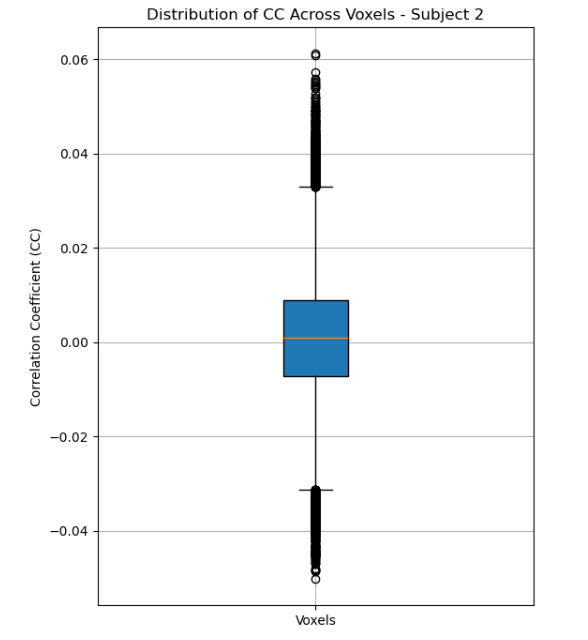
\includegraphics[width=0.5\linewidth]{figs/cc_dist_voxels_subject_2.png}
    \caption{Distribution of CC across voxels for Subject 2 using Bag of Words embeddings.}
    \label{fig:cc_dist_voxels_subject_2}
\end{figure}


\subsection{Stability Analysis}
We conduct a stability analysis by examining performance across different subjects. In this case, we compare Subject 2, which has been detailed so far, with another model trained on Subject 3. We train and test a model on Subject 3 using the same stories as Subject 2. We can then compare the distributions of CCs to see how stable the process is across different subjects.

Our final Subject 3 model uses the Bag of Words embedding and an alpha hyperparameter of 1000 for Ridge. After the training, the final test set performance for Subject 3 was a mean CC of 0.0017, median CC of 0.0014, top 1 percentile CC of 0.0320, and a top 5 percentile CC of 0.0213. This is shown in Table \ref{tab:subject_performance}. In comparison with Subject 2, we note that the top 1 percentile and top 5 percentile CCs are very similar, which suggests stable results. The mean and median CC are better for Subject 3, though not by a large margin that would suggest high instability.

\begin{table}[ht]
  \centering
  \caption{Test Performance Metrics for Subject 2 and Subject 3}
  \label{tab:subject_performance}
  \begin{tabular}{lcccc}
    \hline
    \textbf{Subject} & \textbf{Mean Test CC} & \textbf{Median Test CC} & \textbf{Top 1 Percentile CC} & \textbf{Top 5 Percentile CC} \\
    \hline
    Subject 2        & 0.0009                & 0.0009                 & 0.0311                     & 0.0215                      \\
    Subject 3        & 0.0017                & 0.0014                 & 0.0320                     & 0.0213                      \\
    \hline
  \end{tabular}
\end{table}

We also visualize the distribution of CC across voxels to have a deeper understanding and comparison with Subject 2. This is shown in Figure \ref{fig:cc_dist_voxels_subject_3}. Visually, the distributions of CC across voxels look very similar between Subject 2 and Subject 3. The medians and quartiles, and outliers also show no major differences. This suggests a generally stable result.

\begin{figure}
    \centering
    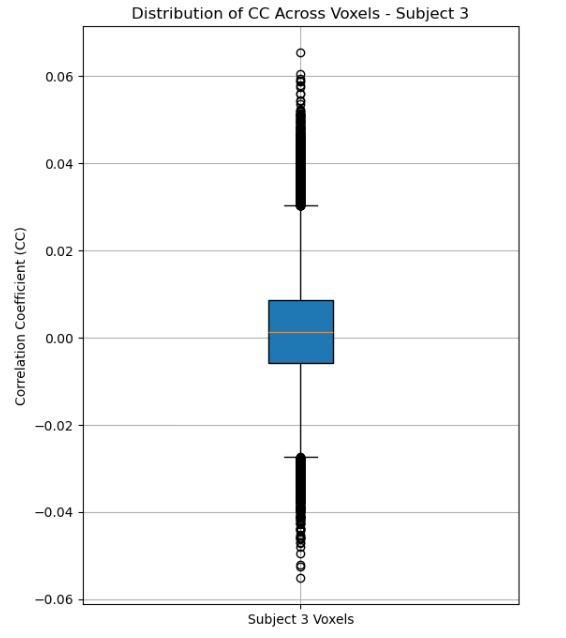
\includegraphics[width=0.5\linewidth]{figs/cc_dist_voxels_subject_3.png}
    \caption{Distribution of CC across voxels for Subject 3 using Bag of Words embeddings.}
    \label{fig:cc_dist_voxels_subject_3}
\end{figure}


\section{Modeling - Encoder Embedding}

In this section, we now fit a linear model using the embeddings generated from the BERT-style encoder, as opposed to the pretrained embeddings. Doing so will allow us to examine if using an encoder shows potential for better predictions than pretrained embeddings, and how they differ. We follow a similar cross validation process testing values across the 0.1 - 1000 range for the Ridge hyperparameter alpha.

\subsection{Encoder Embedding Model - Hyperparameter Selection}
We utilized the same cross validation strategy as in the previous section. The hyperparameter training results for selecting the alpha value are shown in Table \ref{tab:encoder_cv}. Based on the CC scores, we selected alpha=1000 as the best value.

\begin{table}[ht]
\centering
\caption{Performance metrics for encoder embeddings at different values of $\alpha$. Best alpha: 1000 (Mean CV CC = $-0.0052$).}
\label{tab:encoder_cv}
\begin{tabular}{rrrrrr}
\toprule
\textbf{Alpha} & \textbf{Mean CC} & \textbf{Median CC} & \textbf{Top1 CC} & \textbf{Top5 CC} & \textbf{Top10 CC} \\
\midrule
0.1   & -0.0055 & -0.0060 & 0.0382 & 0.0233 & \multicolumn{1}{c}{--} \\
1     & -0.0055 & -0.0060 & 0.0382 & 0.0233 & \multicolumn{1}{c}{--} \\
10    & -0.0056 & -0.0060 & 0.0382 & 0.0233 & \multicolumn{1}{c}{--} \\
100   & -0.0052 & -0.0058 & 0.0393 & 0.0240 & \multicolumn{1}{c}{--} \\
1000  & -0.0052 & -0.0058 & 0.0393 & 0.0240 & \multicolumn{1}{c}{--} \\
\bottomrule
\end{tabular}
\end{table}

\subsection{Encoder Embedding Model - Results}

On the test set, the best model for the encoder embedding (with alpha=1000) reached a mean CC of 0.0060 for Subject 2 and a mean CC of 0.0114. Interestingly, for the encoder embeddings, we see not only significantly greater performance overall but also a larger difference in magnitude between the CC of Subject 2 and Subject 3, which will be examined in further depth. These results are shown in Table \ref{tab:cc_pretrained_vs_encoder_comparison}.


\begin{figure}[ht]
    \centering
    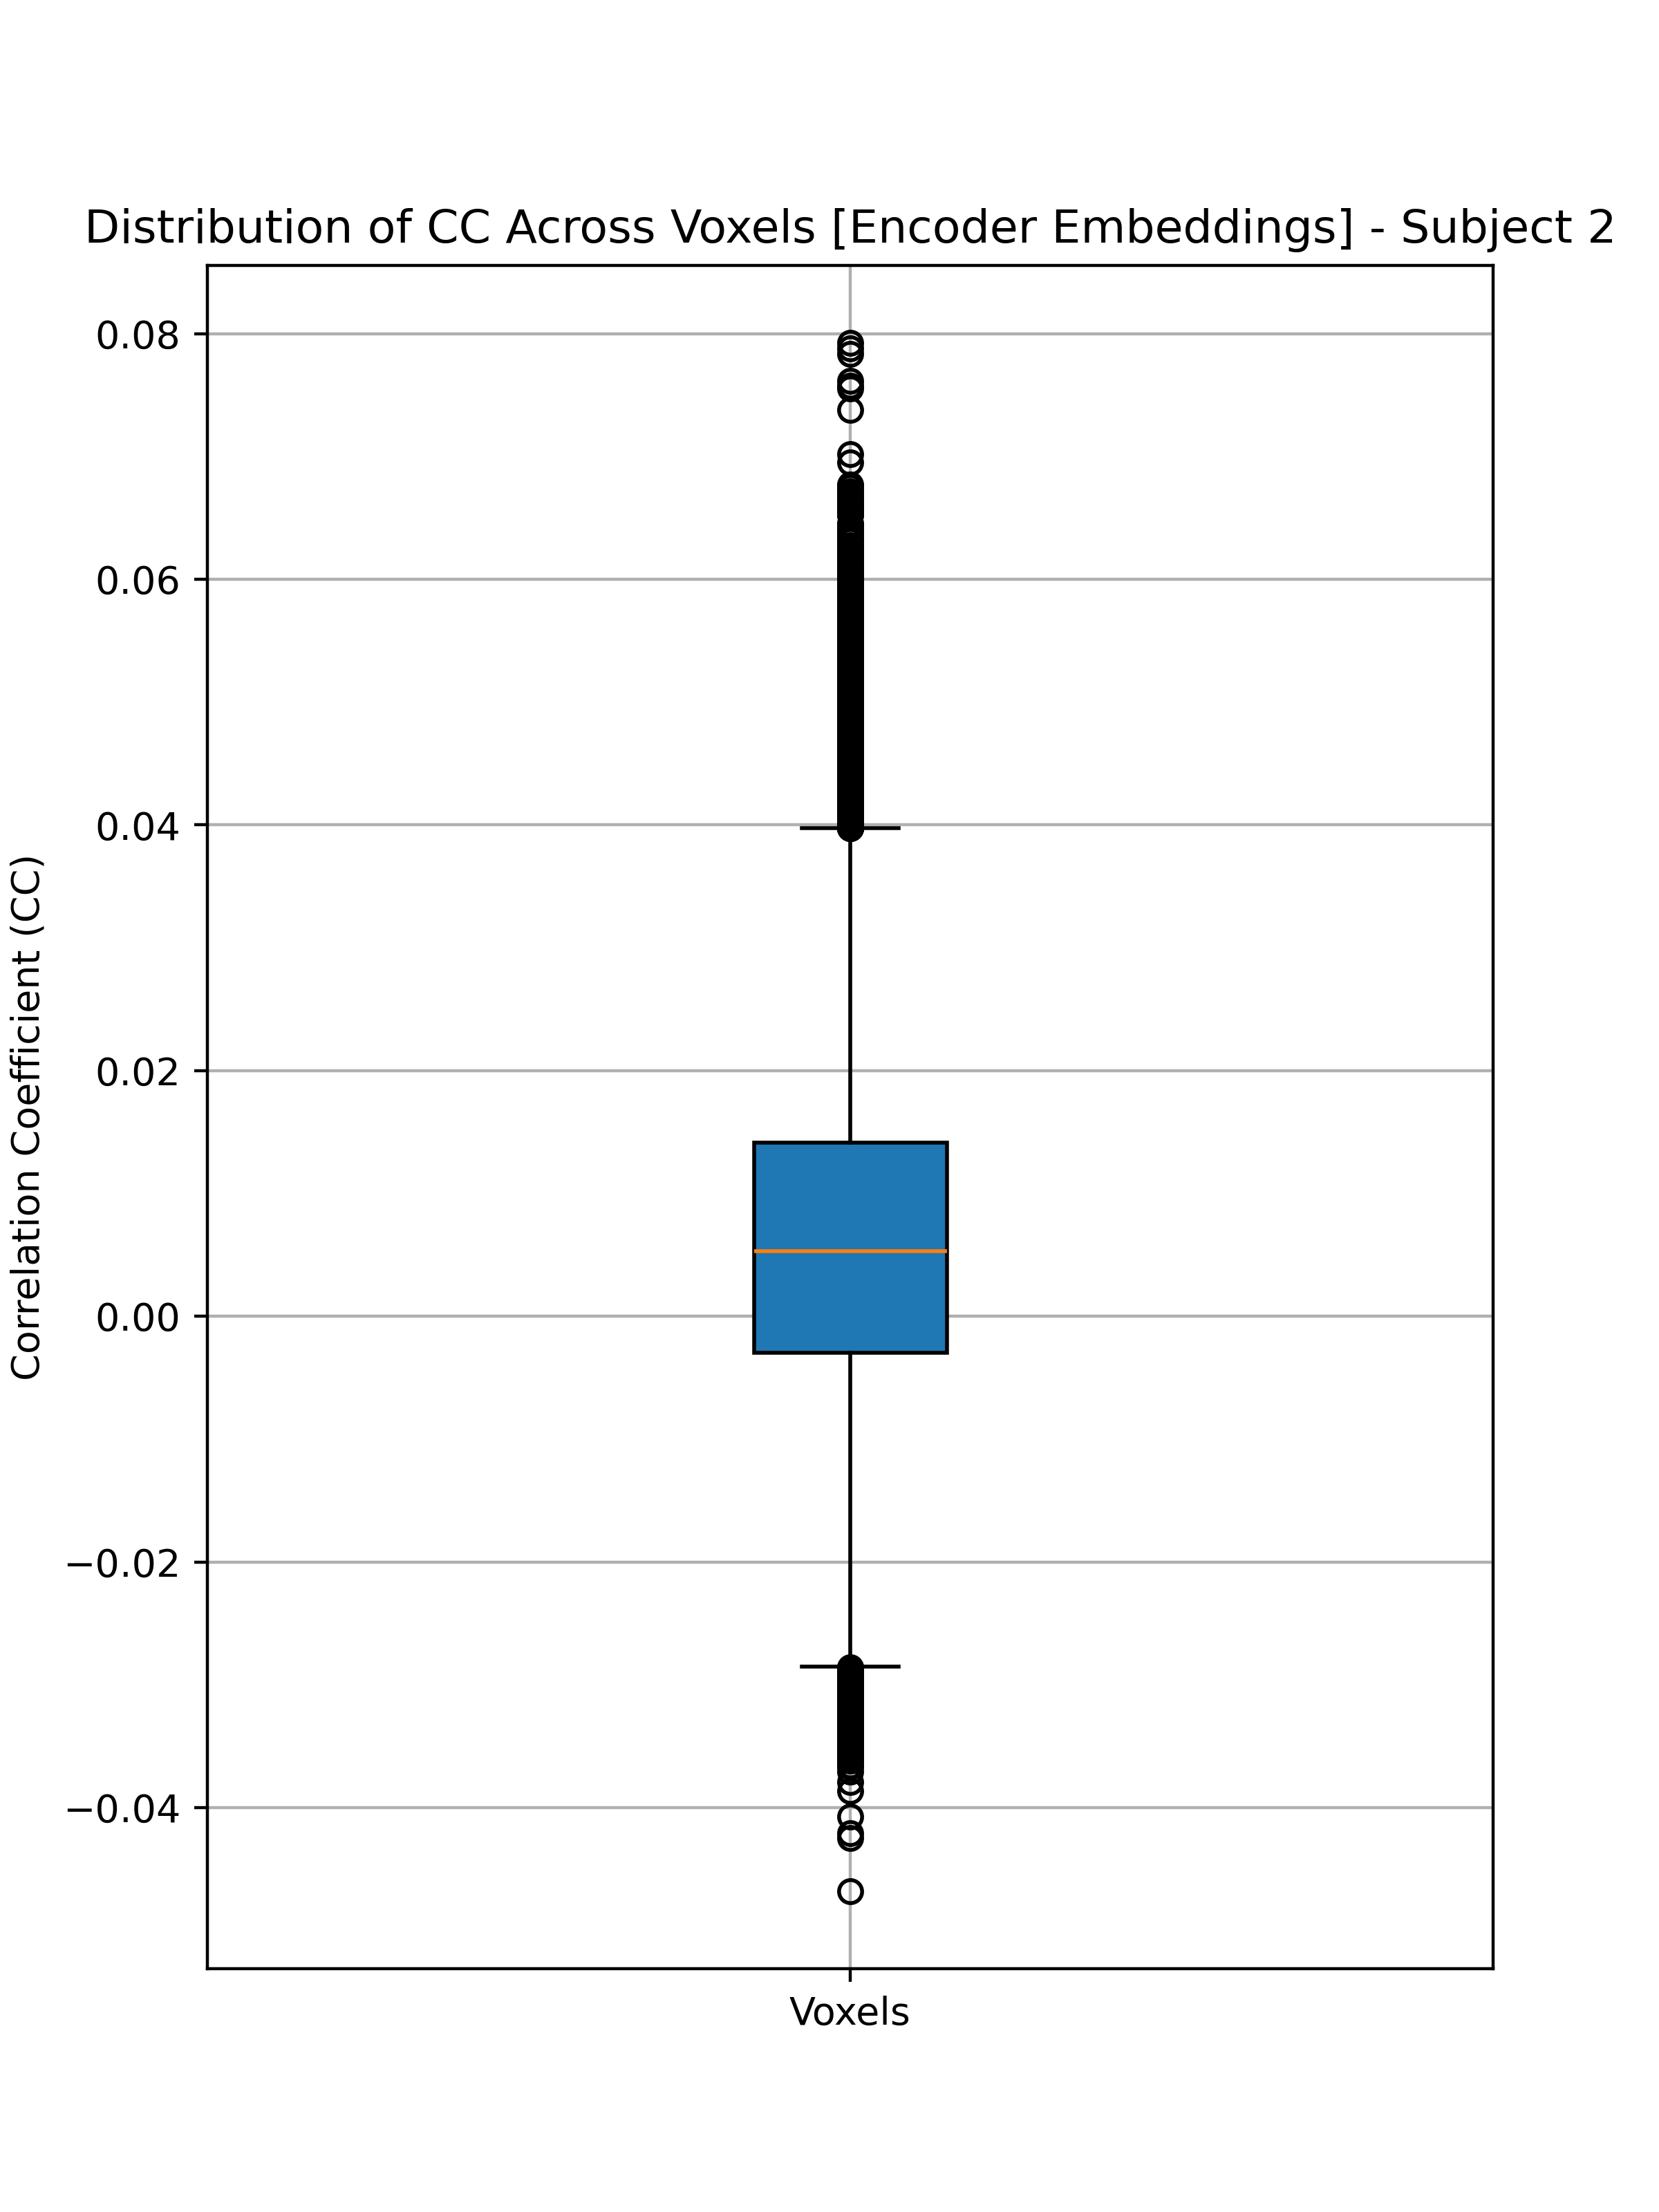
\includegraphics[width=0.5\linewidth]{figs/encoder_subj2_cc_dist.png}
    \caption{Distribution of CC across voxels for Subject 2 using Encoder embeddings.}
    \label{fig:cc_dist_encoder_subject_2}
\end{figure}

\subsection{Encoder Embedding Model - Detailed Evaluation \& Analysis}
We examine the distribution of test CC for the encoder embedding Ridge model across voxels. Figure \ref{fig:cc_dist_encoder_subject_2} describes the distribution of CC across voxels for Subject 2. We can see that the distribution is somewhat symmetric, with a slight upward skew. Numerically, the distribution of CC is centered around 0.007, with a 25th percentile around -0.01 and a 75th percentile at approximately 0.04. An important note is that there are numerous outlier voxels on either side (based on the 1.5*IQR outlier threshold), which suggests that the spread of CC across voxels is relatively large. The positive outliers are more numerous and stronger/further from the center than the negative outliers, reflecting a slight upward skew. One interesting note is that this distribution of CC is generally shifted more upward than the pre-trained embedding (i.e., Bag of Words) model, and has more positive outliers.

So, this model does not perform the same across all voxels, just as we saw with the model using pre-trained embeddings. Scientifically, this implies that prediction in different voxels of the brain has varying levels of difficulty. This could stem from that some brain areas (voxels) are irreverent from language processing, or at least language processing in listening to these stories, leading to noise that cannot be predicted with the story text, while some others actively respond to the story. To investigate this further, more domain knowledge would be useful.

As stated earlier, we want to have a reasonable interpretation criterion for interpreting voxels according to PCS. We want to make sure that the predictions are meaningfully better than by chance. One option is to only select voxels in the top \(x\) percentile of the observed distribution of CCs (i.e., for \(x=5\) for the 5th percentile). The reason to select the top voxels is that we know they respond to the stories actively, while others could be just random noise, as stated before. In terms of stability, we would ideally want to be able to predict voxels well across different stories, subjects, etc. We could check this by examining each voxel's CC across model performance for different stories, or different models for different subjects. Lastly, we want the full prediction process to be reproducible and computed reliably. These conditions align with the three main parts of PCS.


\subsection{Pre-Trained vs. Encoder Embeddings Comparison}

We compare the results of the encoder embedding against the pre-trained embeddings by examining the CC of the encoder model and the Bag of Words model (which was the best pre-trained model). We see that the encoder embeddings are able to reach a higher CC. This is true across all thresholds of CC, including mean, median, Top 1\%, and Top 5\% CC. In particular, the top performance of voxels (for Top 1\% and Top 5\% are closer) is closer, while the mean and median CCs are much higher for the model using encoder embeddings. This can mean that the encoder embeddings generally provide better performance throughout more voxels, whereas the pre-trained embeddings only provide comparable performance at their best voxels. As mentioned, the distribution of CC is generally shifted more upward for the encoder embedding than the pre-trained embedding (i.e., Bag of Words) model, and has more positive outliers. This is shown when comparing the boxplots of the CC distribution across voxels in Figures \ref{fig:cc_dist_voxels_subject_2} and \ref{fig:cc_dist_encoder_subject_2}.

In summary, different embedding methods do not perform equally well across the voxels. The encoder embeddings tend to have better performance across more voxels, whereas the pre-trained embeddings tend to have far worse performance for most voxels. However, the pre-trained embeddings still provide comparable performance to the encoder embeddings for the top-performing voxels for both models.


\begin{table}[ht]
\centering
\caption{Comparison - Test Performance Metrics for Bag-of-Words vs. Pre-Trained Embeddings}
\label{tab:cc_pretrained_vs_encoder_comparison}
\begin{tabular}{llrrrr}
\toprule
\textbf{Embedding}   & \textbf{Subject} & \textbf{Mean CC} & \textbf{Median CC} & \textbf{Top 1 \% CC} & \textbf{Top 5 \% CC} \\
\midrule
Pre-Trained (Bag-of-Words) & 2 & 0.0009 & 0.0009 & 0.0311 & 0.0215 \\
             & 3 & 0.0017 & 0.0014 & 0.0320 & 0.0213 \\
\addlinespace
Encoder      & 2 & 0.0060 & 0.0053 & 0.0416 & 0.0290 \\
             & 3 & 0.0114 & 0.0093 & 0.0681 & 0.0426 \\
\bottomrule
\end{tabular}
\end{table}


\subsection{Encoder Embedding Model - Stability Analysis}
We conduct a stability analysis for the encoder embedding model by examining performance across different subjects. In this case, we compare Subject 2, which has been discussed so far, with another model trained on Subject 3. We train and test a model on Subject 3 using the same stories as Subject 2. We can then compare the distributions of CCs to see how stable the process is across different subjects.

Our final Subject 3 model uses an alpha hyperparameter of 1000 for Ridge. After the training, the final test set performance for Subject 3 was a mean CC of 0.0114, median CC of 0.0093, top 1 percentile CC of 0.0681, and a top 5 percentile CC of 0.0426. This is shown in Table \ref{tab:cc_pretrained_vs_encoder_comparison}. In comparison with Subject 2, the median and median CCs are significantly better for Subject 3, as they are almost double that of Subject 2. The top 1 percentile and top 5 percentiles are closer, though still show a noticeable gap.

We also visualize the distribution of CC across voxels to have a deeper understanding and comparison with Subject 2. This is shown in Figure \ref{fig:cc_dist_encoder_subj_3}. Visually, the distributions of CC across voxels look somewhat similar between Subject 2 and Subject 3, as the medians and quartiles are comparable. However, Subject 3 shows a much stronger right skew and has stronger and more numerous outliers in the higher CC value region. This suggests that Subject 3 has many better, higher-performing voxels. Overall, the differences suggest that there may be some moderate instability in the result of the encoder embedding model across subjects, so further stability testing could be useful.

\begin{figure}[ht]
    \centering
    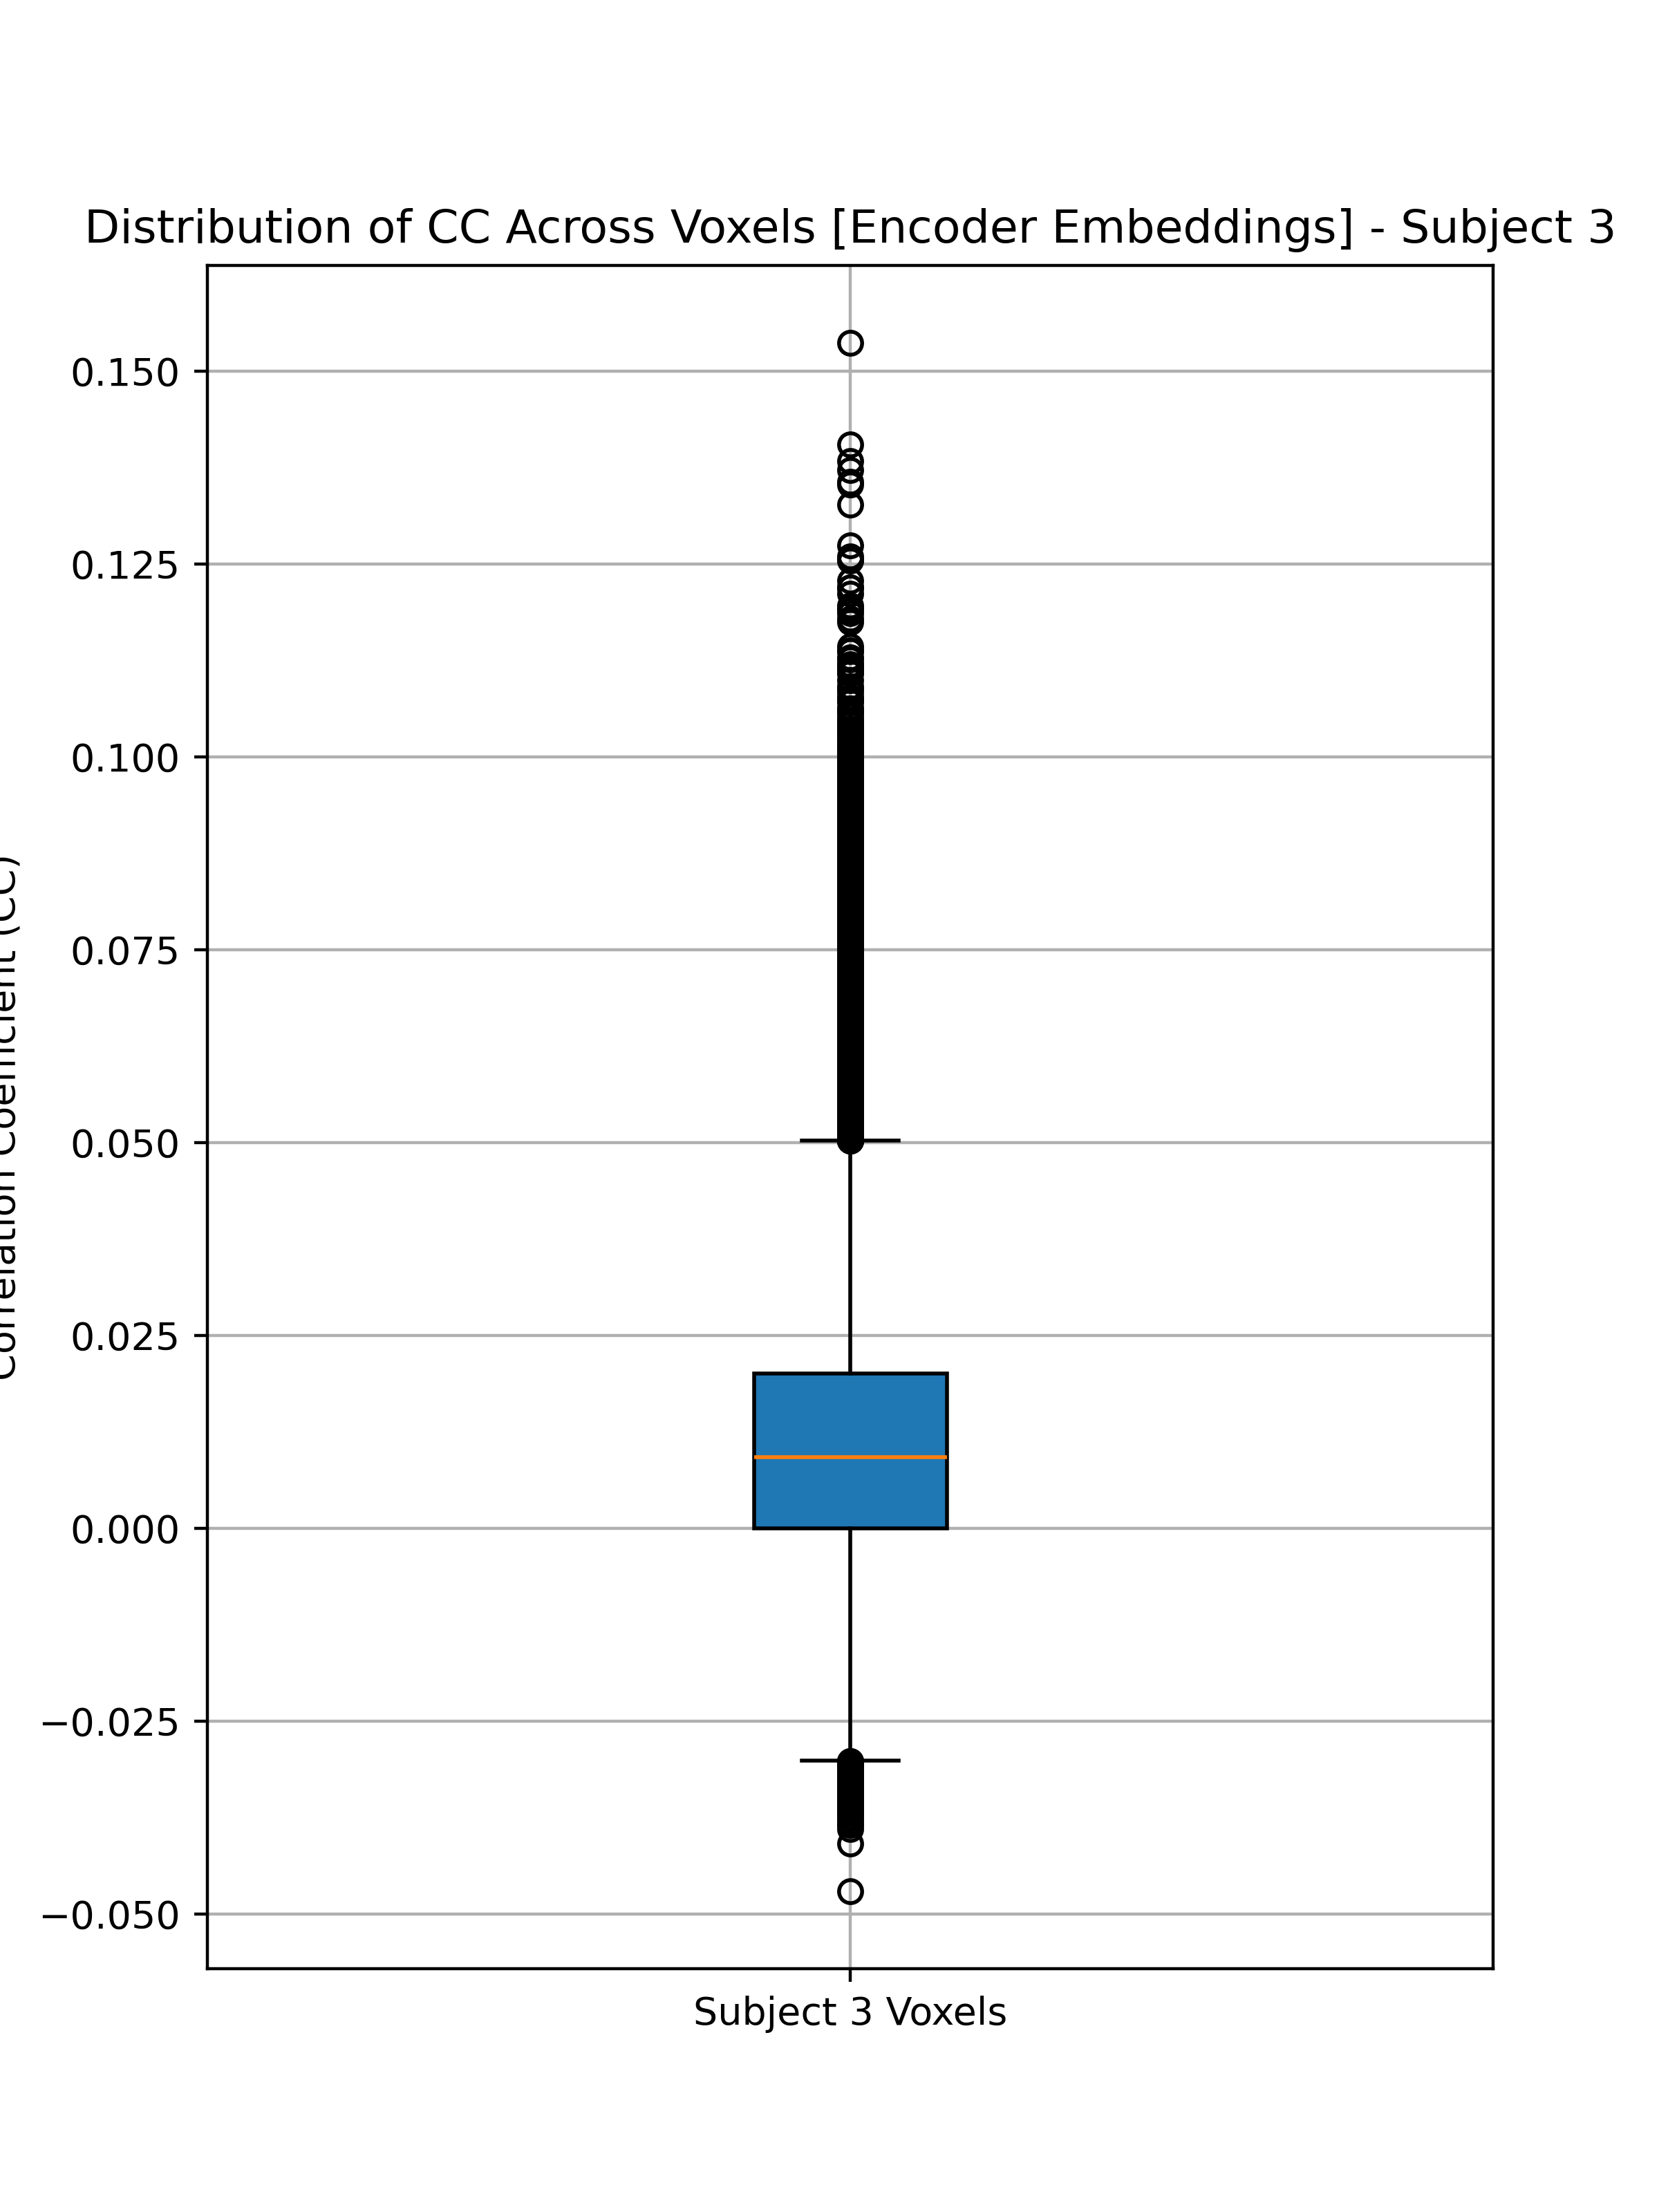
\includegraphics[width=0.5\linewidth]{figs/encoder_subj3_cc_dist.png}
    \caption{Distribution of CC across voxels for Subject 3 using Encoder embeddings.}
    \label{fig:cc_dist_encoder_subj_3}
\end{figure}

\section{Conclusion}
In this lab, we explored the feasibility of predicting fMRI BOLD signals associated with listening to narrative stories using features derived from the story text. We implemented a pipeline that involved generating word-level embeddings using three distinct pre-trained methods: Bag-of-Words, pre-trained Word2Vec, and pre-trained GloVe. These word embeddings were then aggregated to match the fMRI TRs via Lanczos resampling, and temporally lagged features were incorporated to account for the delay and contextual processing. Following this, we also generated embeddings from a BERT-style encoder trained on these stories. Finally, Ridge Regression models were trained for each embedding type to predict voxel-level activity, with performance evaluated using cross-validation and correlation CC.

Our results indicated that predicting fMRI signals with this approach is challenging, yielding generally low CC values across all models, suggesting limited predictive power. Surprisingly, the semantically simple BoW model outperformed the models based on pre-trained Word2Vec and GloVe embeddings, achieving the highest average CC during cross-validation, albeit still at a low absolute level. Further analysis of the best-performing BoW model revealed variability in prediction accuracy across different brain voxels, though the overall performance patterns showed reasonable stability when compared across the two subjects.

Among the pre-trained embeddings, the weak performance, particularly of the semantically meaningful Word2Vec and GloVe embeddings, points towards a fundamental limitation in relying solely on aggregated word embeddings linearly. Language resampling is additive; the meaning of a sentence is far more complex than a simple linear combination of its constituent word meanings. Operations like negation (e.g., the word "not" altering meaning) or the context-dependent meaning of words are not well captured by linearly averaging pre-computed word vectors using Lanczos resampling. The better performance of BoW in this specific pipeline might stem from several factors. Firstly, its high dimensionality might preserve more distinct information than low-dimensional dense vectors of Word2Vec/GloVe. Secondly, because BoW embeddings don't encode complex inter-word semantics initially, the linear averaging process might be less detrimental to the simpler information (word presence/frequency) they convey. In essence, the combination of linear aggregation (Lanczos) and a linear predictive model (Ridge) appears ill-suited to leverage the strengths of dense semantic embeddings. This suggests that more sophisticated methods capable of handling non-linear aggregation and context are likely necessary to effectively model the brain's processing of natural language.

The BERT-style encoder embedding resulted in a stronger performance than the pre-trained embeddings, which is particularly remarkable given its low dimensionality (32/64) compared to the pre-trained embeddings (more than 5000). This may highlight the encoder's ability to better embed story information in a relevant way. The main reason why this may be the case is that the encoder is able to capture more semantic information in the document level, rather than each treating each word independently, like the pre-trained embeddings. Seeing as the human brains understand the entire story, the contextual information likely aligns better with how do humans process language.
\newpage

\printbibliography

\appendix
\section{Academic honesty}
\subsection{Statement}
We affirm that the work in this report is entirely my own. We have not copied from any unauthorized sources, and all contributions from classmates, external sources, or tools are acknowledged. Academic research honesty is necessary because it ensures fairness, builds trust in scholarly work, and reflects personal integrity. Misrepresenting work undermines academic standards and disrespects the time and effort of peers and educators. Maintaining honesty in research fosters a learning environment where collaboration and progress can thrive authentically.

\subsection{LLM Usage}

We used ChatGPT to assist in clarifying concepts, creating visualizations, checking grammar, and improving the structure of our explanations. No content of the report or code was generated by the LLM without our review, editing, and refinement. We ensured that all content was written and understood by us, and the LLM was used as a tool to enhance our work rather than replace our understanding, we take full responsibility for all content in the report.

\end{document}